% mn2esample.tex
%
% v2.1 released 22nd May 2002 (G. Hutton)
%
% The mnsample.tex file has been amended to highlight
% the proper use of LaTeX2e code with the class file
% and using natbib cross-referencing. These changes
% do not reflect the original paper by A. V. Raveendran.
%
% Previous versions of this sample document were
% compatible with the LaTeX 2.09 style file mn.sty
% v1.2 released 5th September 1994 (M. Reed)
% v1.1 released 18th July 1994
% v1.0 released 28th January 1994

\documentclass[a4paper,useAMS,usenatbib]{mn2e}

\usepackage[pdftex]{graphicx}
\usepackage{amssymb,amsmath}
\usepackage{booktabs}
\usepackage{afterpage}
%\usepackage{pdflscape}

% If your system does not have the AMS fonts version 2.0 installed, then
% remove the useAMS option.
%
% useAMS allows you to obtain upright Greek characters.
% e.g. \umu, \upi etc.  See the section on "Upright Greek characters" in
% this guide for further information.
%
% If you are using AMS 2.0 fonts, bold math letters/symbols are available
% at a larger range of sizes for NFSS release 1 and 2 (using \boldmath or
% preferably \bmath).
%
% The usenatbib command allows the use of Patrick Daly's natbib.sty for
% cross-referencing.
%
% If you wish to typeset the paper in Times font (if you do not have the
% PostScript Type 1 Computer Modern fonts you will need to do this to get
% smoother fonts in a PDF file) then uncomment the next line
% \usepackage{Times}

%%%%% AUTHORS - PLACE YOUR OWN MACROS HERE %%%%%


%%%%%%%%%%%%%%%%%%%%%%%%%%%%%%%%%%%%%%%%%%%%%%%%

\title[Optical cartography of the Northern Galactic Plane]{Optical cartography 
of the Northern Galactic Plane: IPHAS stellar density maps as tests of Galactic models}
\author[H. J. Farnhill et al.]{H. J. Farnhill$^{1}$\thanks{E-mail:
h.farnhill@herts.ac.uk} et al.
\\
$^{1}$Centre for Astrophysics Research, Science and Technology Research Institute, University of Hertfordshire, College Lane, Hatfield, AL10 9AB, U.K.}
\begin{document}

\date{Draft last compiled \today}

\pagerange{\pageref{firstpage}--\pageref{lastpage}} \pubyear{2015}

\maketitle

\label{firstpage}

\begin{abstract}
Galactic models are becoming increasingly powerful tools to interpret the 
large amounts of data produced by the new generation of Galactic Plane 
surveys. In order to test the performance of the Besan\c{c}on model of 
Galactic population synthesis, along with a number of extinction models, 
incompleteness-corrected density maps derived from IPHAS broad-band photometry 
were produced, and are presented here.
\end{abstract}

\begin{keywords}
Galaxy: stellar content -- extinction.
\end{keywords}

\section{Introduction}

The positioning of the Solar System almost in the equatorial plane of the Milky
Way places a significant obstacle in the way of understanding the structure of our 
own galaxy.  Despite the fact that the disc of the Milky Way is effectively 
the largest object in the night sky, offering vastly superior angular resolution 
compared to that achievable for any other galaxy, sightlines at low Galactic latitude 
remain a challenge to decipher because of large and variable amounts of dust 
extinction.  Given that the formation and maintenance of galactic 
discs is an important problem in galaxy evolution (review reference), an improved 
vision of our own galactic disc is needed.  And as our wider home, it is of interest 
in its own right.

The reliable empirical determination of the 3-dimensional distribution of the Milky 
Way's interstellar dust, needed to make sense of the disc, is now becoming possible 
through the increasingly sophisticated analyses of comprehensive digital survey data 
(Drimmel \& Spergel 2002 - check, Marshall et al 2006, Sale et al 2009, 2014).  In the
next 5-10 years, these advances will complement the astrometric harvest being gathered 
by the Gaia mission and usher in a much better, sharper vision of the 3D Galactic disc.
Nevertheless, the anticipated Gaia parallax precision at fainter magnitudes ($100\mu$arcsec 
at $G \sim 19$) will still leave stars beyond the first 1--2 kpc with distances known to 
a precision worse than ~10-20 percent.  Accordingly, it remains useful to supplement 
our knowledge through the application of other methods that can test predictive Galactic 
models.  One of these, that puts to good use the uniquely detailed view we have of the 
Galactic disc, is the exploitation of magnitude-limited star counts.  This approach has 
been applied successfully in the past and it has been influential in both guiding and 
testing the content of Galactic models (Robin et al 2003, Czekaj et al 2014).  

So far, deeper optical star-count mapping has only been carried out in the 
southern Galactic plane (DENIS reference?).  The options to conduct a 
well-calibrated stellar density mapping of the northern sky are now 
appearing with the advent of digital imaging surveys (SDSS, Pan-STARRS - 
refs).  The greater challenge is at low Galactic latitudes, but this is now 
tractable as the 1 arcsec angular-resolution IPHAS (Drew et al 2005), and 
UVEX (Groot et al 2009) surveys approach completion.  In particular, the 
recent release of IPHAS DR2 (Barentsen et al 2014), offering a uniform 
photometric calibration of the northern Galactic Plane in $r$, $i$ (and 
$H\alpha$), provides the basis for a precise and deep stellar density map 
across almost 1800 square degrees.

In this work, we describe the construction of $r$, $i$ stellar density maps at
a range of resolutions, up to a maximum resolution of 1 square arcminute, 
based on IPHAS DR2.  In order that this mapping is not hampered by variable 
observing conditions and similarly variable source losses, great care has been 
taken to make corrections for incompleteness and confusion by evaluating the 
results of artificial source injection tailored to every survey field. Because 
this technical process has so far only been discussed superficially in the 
literature (see e.g. *ref* for the fullest description to date), we present a 
reasonably full description of how we arrive at the position- and 
magnitude-dependent corrections applied.  This is presented in section 3 (after
a brief restatement of the main features of the IPHAS survey in section 2).

The way in which the corrected r, i stellar density maps are assembled is described in 
section 4.  This includes the specifications of the maps and pointers on how to access 
them.  In $i$ band our map reaches down to 18th mag (Vega system), a limit that roughly
corresponds to Gaia G $\sim$ 19 (see Appendix B).   In section 5, the maps are subjected 
to first comparisons with Galactic model predictions.  This is attempted using distinct 
prescriptions of the 3-D distribution of interstellar extinction in order to gain a 
first impression of how influential the choice of 3D extinction map can be.  Interestingly, the 
results from this limited exploration are already mixed: we find that outside the 
Solar Circle ($\ell > 90^{\circ}$  in the north), the agreement between star counts and 
model prediction is quite good -- but at the lowest Galactic longitudes examined, 
significant discrepancies appear.  The paper ends in section 6 with a brief discussion of 
these results and a summary.



% \begin{table*}
%  \centering
%  \begin{minipage}{140mm}
%   \caption{Data on the RV Tauri stars detected by {\it IRAS}.}
%   \begin{tabular}{@{}llrrrrlrlr@{}}
%   \hline
%    Name     &            & \multicolumn{4}{c}{Flux density (Jy)%
%   \footnote{Observed by {\em IRAS}.}}\\
%    Variable & {\it IRAS} & 12$\,\umu$m & 25$\,\umu$m & 60$\,\umu$m
%      & 100$\,\umu$m & Sp. & Period & Light- & $T_0\,(\rmn{K})$ \\
%         &  &  &  &  &  & group & (d) & curve \\
%         &  &  &  &  &  &       &     & type  \\
%  \hline
%  TW Cam & 04166$+$5719 & 8.27 & 5.62 & 1.82 & $<$1.73 & A & 85.6 & a & 555 \\
%  RV Tau & 04440$+$2605 & 22.53 & 18.08 & 6.40 & 2.52 & A & 78.9 & b & 460 \\
%  DY Ori & 06034$+$1354 & 12.44 & 14.93 & 4.12 & $<$11.22 & B & 60.3 &  & 295 \\
%  CT Ori & 06072$+$0953 & 6.16 & 5.57 & 1.22 & $<$1.54 & B & 135.6 &  & 330 \\
%  SU Gem & 06108$+$2734 & 7.90 & 5.69 & 2.16 & $<$11.66 & A & 50.1 & b & 575 \\
%  UY CMa & 06160$-$1701 & 3.51 & 2.48 & 0.57 & $<$1.00 & B & 113.9 & a & 420 \\
%  U Mon  & 07284$-$0940 & 124.30 & 88.43 & 26.28 & 9.24 & A & 92.3 & b & 480 \\
%  AR Pup & 08011$-$3627 & 131.33 & 94.32 & 25.81 & 11.65 & B & 75.0 & b & 450 \\
%  IW Car & 09256$-$6324 & 101/06 & 96.24 & 34.19 & 13.07 & B & 67.5 & b & 395 \\
%  GK Car & 11118$-$5726 & 2.87 & 2.48 & 0.78 & $<$12.13 & B & 55.6 &  & 405 \\
%  RU Cen & 12067$-$4508 & 5.36 & 11.02 & 5.57 & 2.01 & B & 64.7 &  & 255 \\
%  SX Cen & 12185$-$4856 & 5.95 & 3.62 & 1.09 & $<$1.50 & B & 32.9 & b & 590 \\
%  AI Sco & 17530$-$3348 & 17.68 & 11.46 & 2.88 & $<$45.62 & A & 71.0 & b & 480 \\
%  AC Her & 18281$+$2149 & 41.47 & 65.33 & 21.12 & 7.79 & B & 75.5 & a & 260 \\
%  R Sct  & 18448$-$0545 & 20.88 & 9.30 & 8.10 & $<$138.78 & A & 140.2 & a \\
%  R Sge  & 20117$+$1634 & 10.63 & 7.57 & 2.10 & $<$1.66 & A & 70.6 & b & 455 \\
%  V Vul  & 20343$+$2625 & 12.39 & 5.72 & 1.29 & $<$6.96 & A & 75.7 & a & 690\\
% \hline
% \end{tabular}
% \end{minipage}
% \end{table*}

\section[]{Observations}

\subsection{IPHAS broad-band photometry}

The most recent release, DR2, of the INT/WFC Photometric H$\alpha$ Survey of the Northern Galactic Plane (IPHAS) was 
presented by Barentsen et al (2014), while the basic specification of IPHAS was set down by Drew et al (2005).  This 
survey, conducted using the Wide Field Camera (WFC) mounted on the Isaac Newton Telescope (INT) in La Palma, provides 
photometry of the complete Northern Galactic Plane within the latitude range $-5^{\circ} < b < +5^{\circ}$, in narrow-band 
H$\alpha$ and broadband Sloan $r$ and $i$.  It is the broadbands that are the focus of this paper.  The typical 
$5\sigma$ magnitude limit reached in the survey is 21.2 in $r$ and 20.0 in $i$, achieved at a median seeing of 1.1 arcsec.  
The typical external photometric precision of DR2 is close to 0.03 magnitudes, as judged by comparisons with SDSS DR9 
data.  In Galactic longitude terms this survey spans the range $30^{\circ} < \ell < 215^{\circ}$.  In time it will be 
fully complemented by the VPHAS+ survey (Drew et al 2014) covering the Southern Galactic Plane and Bulge.  

Whilst IPHAS is certainly uniform in its execution, the weather at the telescope represented an important variable.  The 
observations were obtained via standard allocations of time, with the result that a wide variety of observing conditions 
are contained within the survey database.  Thanks to the opportunity to obtain repeats of fields exposed in poor conditions, 
it was possible to apply quality cuts in the preparation of IPHAS DR2 so as to omit clearly inferior data, whilst still 
achieving over 92\% coverage of the survey footprint.  Even so, there is still a broad quality range within DR2 in terms 
of both measured widths of the point spread function (PSF), and limiting magnitude (for full details, 
see \citet{Barentsen2014}).  This variation, along with over a factor of ten constrast in the typical observed stellar density along the Northern 
across the northern Plane (see figure 3 in \citet{Gonzalez-Solares2008}), makes it important to 
achieve uniformity of outcome and well-defined errors through careful position-dependent completeness corrections. 
This task, along with the development and application of an algorithm that ensures reliable source 
counting without duplication and proper accounting for small gaps and other irregularities in the data, is the work 
presented here (see also Farnhill 2015, PhD Thesis).

The first step in this process is to establish a working definition of a detected 'star' in the survey data.


\subsection{On morphological classification and the expected number density of extra-galactic sources}
\label{subsec:galaxy_density}

A fraction of sources detected in DR2 fields are known to be misclassified as 
non-stellar towards field edges - this is due to progressive distortion in the PSF with increasing 
distance from the optical axis (OA) of the INT/WFC system. This pattern of behaviour has a small 
impact on the final DR2 catalogues, which provide primary detections that are selected according to 
a criterion of lowest distance to the optical axis.  But when counting stellar (morphological class -1) 
sources from a single field to produce a stellar density map the issue of progressive misclassification 
has to be tackled. Fig. \ref{fig:misclassification} shows an example of a field exhibiting this problem.

\begin{figure}
\begin{center}
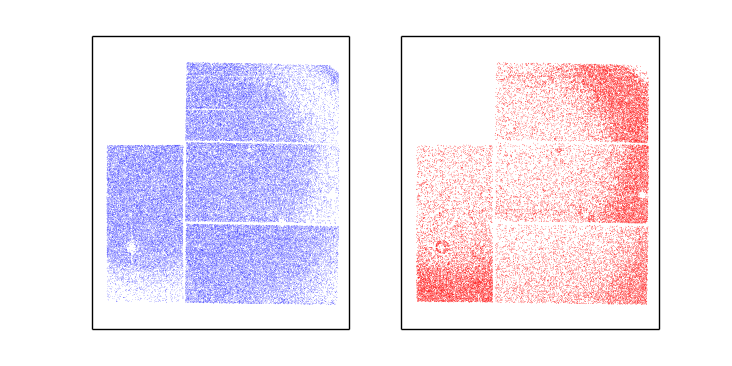
\includegraphics[width=1\linewidth]{figures/morphology_misclassification.png} 
\caption{\footnotesize{Distributions of sources classified as stellar ($rClass=-1$, blue) 
and non-stellar ($rClass=+1$, red) in the $r^{\prime}$-band for IPHAS field 4975o\_aug2004a} }
\label{fig:misclassification}
\end{center}
\end{figure}

Assuming a constant ratio of stellar to non-stellar sources applies in reality across 
any one field, comparisons between 5 sq. deg. regions at field centres and edges revealed
occasional misclassification of several hundred sources. Of course, some of these objects 
are not misclassified -- they can be genuine examples of galaxies presenting as extended objects.  
To determine the expected number of galaxies detected in a similar area, galaxy counts were 
taken from \citet{Yasuda2001}, down to the 5$\sigma$ $r^{\prime}$- and $i^{\prime}$-band limits 
of IPHAS, and then extinguished by the median \citet{Schlegel1998} extinction values for all fields 
(corrected using the \citet{Schlafly2011} recalibration). Based on median limiting magnitudes, 
$\sim 1$ extragalactic source is predicted per 5 sq. deg. region. Against stellar densities typically 
orders of magnitude larger, this is very small.  It was therefore regarded as safe to include 
'non-stellar' +1 classified sources for density mapping purposes - the losses that would be 
suffered on leaving them out, in fields similar to that depicted in Fig. \ref{fig:misclassification}, 
are much larger than is the likely contribution from galaxies.

% In the case where all point sources are accurately classified, the primary
% source of extended objects would be galaxies - only a smaller fraction would be
% contributed by Galactic sources with extended emission e.g. planetary nebulae
% and WR stars. Such Galactic contributions would be sufficiently small - such
% rare objects' number densities amount to an average of $<$1 object per IPHAS
% field \citep{Sabin2014, Stock2010} - that they would have negligible impact on
% density mapping efforts if included in stellar number counts. The inclusion of
% galaxies needs further thought, as the apparent density of galaxies varies
% considerably across the sky.

% Due to the misclassification effect demonstrated in Fig.
% \ref{fig:morphology_misclassification}, a certain fraction of objects are
% rendered indistinguishable from galaxies on the basis of their morphology code
% alone. To aid in the decision of whether or not to exclude objects assigned the
% morphology class $+1$, the difference in this fraction between affected and non-
% affected (i.e. the optical axis) regions of the image plane was determined.

% \begin{table*}
% \centering\begin{tabular}{r|ccc|ccc}
% \toprule
% & \multicolumn{3}{|c|}{Optical Axis} & \multicolumn{3}{|c}{CCD3} \\
% Field & -1 & +1 & \% non-stellar & -1 & +1 & \% non-stellar \\
% \midrule
% 4975o\_aug2004a & 437 & 139 & 24.13\% & 62 & 439 & 87.62\% \\
% 0105\_aug2004a & 110 & 53 & 32.52\% & 6 & 152 & 96.20\% \\
% 7474\_dec2006 & 75 & 36 & 32.43\% & 15 & 80 & 84.21\% \\
% 0310\_dec2005 & 330 & 72 & 17.91\% & 227 & 67 & 22.79\% \\
% \bottomrule
% \end{tabular}
% \caption{\footnotesize Numbers of objects appearing as stellar ($rClass=+1$) 
% and non-stellar ($rClass=-1$) in 5 sq. arcmin. regions at the optical axis 
% of the field and towards the vignetted region in CCD3. The first three fields 
% suffer from misclassification issue to varying degrees, while the fourth does 
% not. The shift towards classifying objects as non-stellar at the outskirts of 
% a pointing is illustrated in Fig.. \ref{fig:morphology_misclassification}.}
% \label{table:morphology_misclassification}
% \end{table*}

% Table \ref{table:morphology_misclassification} shows the extent of the
% misclassification illustrated in Fig. \ref{fig:morphology_misclassification},
% along with other examples. The numbers quoted are for regions of area 5 sq.
% arcmin.. In the most extreme case investigated, shown in Fig.
% \ref{fig:morphology_misclassification}, assuming that the $\dfrac{stellar}{non-
% stellar}$ ratio remains roughly constant across the field, an estimated
% $\sim$300 objects are construed as misclassified in the CCD3 region. If this
% density of objects is much greater than the expected density of genuine non-
% stellar sources, then the losses from eliminating $rClass=+1$ objects from
% counts would be more damaging than the uncertainties introduced by retaining
% them in a sample of point sources. Galaxies are the primary source of extended
% objects. Hence a comparison between the estimated misclassification rate and
% expected number densities of galaxies will aid in the decision as to whether or
% not to permit $rClass=+1$ objects to remain in our sample.

% \citet{Yasuda2001} investigated galaxy number counts using early data from
% SDSS, making observations towards the Galactic caps. By visually inspecting
% galaxies towards the northern Galactic cap up to $r^{\prime}=16$, and then
% switching to automated object classification at fainter magnitudes, they counted
% 764,335 galaxies in the $r^{\prime}$-band, and 716,099 in the $i^{\prime}$-band.
% The values for each magnitude bin are listed in Table \ref{table:yasuda} and are
% plotted in Fig. \ref{fig:yasuda}, after they have been scaled to the area of a
% WFC CCD. Over such an area, on average, $\approx$350 galaxies would be expected
% in both the $r^{\prime}$ and $i^{\prime}$-band down to the limiting magnitude of
% the Yasuda sample (21.5). This would be the case if the extinction in the
% direction of IPHAS fields were the same as that of the observations by
% \cite{Yasuda2001}. However their observations, towards the northern Galactic
% cap, experienced $E(B-V)<0.1$ - significantly lower than the typical integrated
% extinction along sightlines in the Galactic plane.

% The median $A_{r^{\prime}}$ for all IPHAS fields from the \citet{Schlegel1998}
% map corrected according to \citet{Schlafly2011} is 2.64 mag, and
% $A_{i^{\prime}}=1.97$ mag. Here the colour excess $E(B-V)$, derived from the
% \citet{Schlegel1998} map using the central coordinates of each IPHAS field, is
% taken to represent the extinction for entire fields. Taking the 5$\sigma$ depths
% of IPHAS of $r^{\prime}=21.2$ and $i^{\prime}=20.0$ \citep{Barentsen2014}, the
% median limiting magnitudes after applying the median
% $A_{r^{\prime}}$/$A_{i^{\prime}}$ are $r^{\prime}=18.56$ and $i^{\prime}=18.03$.
% The cumulative count of \citet{Yasuda2001} galaxy counts down to these limits
% are $<$20 in both $r^{\prime}$- and $i^{\prime}$- bands. For a region of 5 sq.
% arcmin. as considered in Table \ref{table:morphology_misclassification}, the
% estimated galaxy count is $\lesssim$1 - insignificant compared to potentially
% misclassified point sources (see Table
% \ref{table:morphology_misclassification}).

% \begin{figure}
% \begin{center}
% 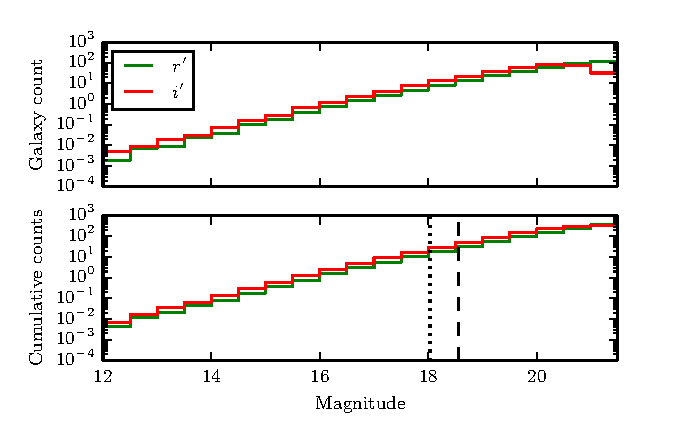
\includegraphics[width=1\linewidth]{figures/yasuda.pdf} 
% \caption{\footnotesize{Galaxy counts vs. magnitude from \cite{Yasuda2001}.
% Normalized counts (originally 0.5 mag deg$^{-2}$) have been scaled to effective
% WFC CCD area. \textbf{Vertical dashed line:} the 5$\sigma$ limit of IPHAS
% $r^{\prime}$-band detections (21.2 mag) less the median $A_{r^{\prime}}$ of
% IPHAS fields taken from the \citet{Schlegel1998} extinction map (2.64 mag, after
% applying correction factor of \citet{Schlafly2011}). \textbf{Dotted line:} the
% same but for $i^{\prime}$, with a 5$\sigma$ limit of 20.0 mag and a median
% $A_{i^{\prime}}=1.97$ mag.}}
% \label{fig:yasuda}
% \end{center}
% \end{figure}

% Based on these estimated extragalactic source counts it was obvious that in
% situations where accurate overall IPHAS source counts are needed, a far larger
% impact would be felt by excluding +1 classed sources (potentially losing
% hundreds of misclassified sources in the process) compared to admitting them,
% thereby counting a small number of galaxies.


\section[]{Completeness correction} 
\label{sec:completeness}

Genuine astronomical sources falling within IPHAS detection limits can fail to
appear in the resulting photometric catalogues for a number of reasons.   Detector issues can 
prevent sources from being picked up: the WFC is a 4-CCD mosaic leaving gaps
between the component detectors, and there are also bad columns and regions of
vignetting that will hinder detection. In the majority of such cases (but not quite all),
missing sources will be picked up in the offset partner pointing, or in the overlap with a 
neighbouring field.

More significant and pervasive losses affecting the final star counts are those
due either to confusion promoted by high stellar densities or to statistical sensitivity losses at the 
faint limit for detection.  In the Galactic plane at lower longitudes, where the stellar density in 
IPHAS can reach up to 500,000 per square degree, confusion will be especially important and liable to 
determine the effective magnitude limit.  Outside the Solar Circle where the typical stellar density is 
50,000 per square degree, confusion is no more than marginally significant: the median 1.1 arcsec PSF 
implies 70 'beams' per source, to be compared with the rule of thumb confusion threshold of 30 per 
source (see Hogg 2001).   Both kinds of incompleteness are exacerbated by relatively poor seeing.  We 
first consider confusion and its estimation in some detail, before going on to describe our chosen 
method of incompleteness correction based on artifical source injection.

\subsection{Confusion, as estimated from the nearest-neighbour distribution}

Confusion, the effect of background noise caused by unresolved sources, scales with source density \citep{Condon1974}. 
For randomly distributed sources, the probability of finding a given number of neighbours within a certain 
distance can be described by a Poisson distribution, which leads to the nearest neighbour distribution 
\begin{equation}
n(\theta) = 2\rho^2\Omega\pi\theta\mathrm{e}^{-\rho\pi\theta^2}
\label{eq:theoretical_neighbours}
\end{equation}
\noindent as presented in \citet{Bahcall1986}.

Fig. \ref{fig:theoretical_neighbours} shows this distribution for an area with the effective area of the WFC field of 
view (0.29 sq. deg.) containing varying numbers of sources. It can be seen that increasing the density of sources 
increases the number of nearest neighbours at small separations, while suppressing the number at greater separations,
thereby pulling in the peak separation value, $\theta_{max}$.  Equation~\ref{eq:theoretical_neighbours} holds for a 
population of sources randomly 
distributed regardless of brightness. In practice, where the distribution of source brightnesses is described by a 
power law, the susceptibility of a source to confusion increases with decreasing brightness: a limiting faint magnitude 
must be chosen in order to define a meaningful confusion rate.


% \citet{Hogg2001} quote a
% rule-of-thumb  that states \textit{``''confusion becomes important at 1/30 of a
% source per beam''}. In the language of optical observations, a beam corresponds
% to the area traced out by the typical PSF of an image, taken by \citet{Hogg2001}
% to be the area defined by a circle with a radius of 1$\sigma$ of the Gaussian
% PSF (of FWHM $\theta_{\mathrm{FWHM}}$ of an image. Using their derived
% expression for the solid angle of a "beam"
% \begin{equation}
% \Omega_{\mathrm{beam}} = \frac{\pi\theta_{\mathrm{FWHM}}^2}{8\ln(2)}
% \label{eqn:hogg}
% \end{equation}
% \noindent and a seeing of 1.8$^{\primeprime}$ - slightly above average for IPHAS
% \observations - gives an $\Omega_{\mathrm{beam}}$ of 1.83 sq. arcsec.. Taking the
% \highest densities seen in the maps produced in Chapter \ref{ch:IPHASDM}
% ($\approx$200 sources / sq. arcmin.), this yields $\approx$0.1 sources per "beam"
% - higher than the 1/30 figure at which confusion starts to become important.

% The effect of source confusion (particularly a problem in the redder
% $i^{\prime}$-band filter and in dense fields) can be estimated based on the fact
% that for stars randomly distributed on an image, the distance of their nearest
% neighbours can be described by a Poisson distribution. The probability of
% finding $x$ neighbours within an angular distance $\theta$ of a star is
% estimated to be
% \begin{equation}
% P(x) = \frac{\mu^x}{x!}\mathrm{e}^{-\mu}
% \end{equation}

% \noindent where $\mu=\rho\pi\theta^2$ (the expected number of sources within the
% area $\pi\theta^2$, with $\rho$ giving the density of stars per unit solid angle).
% The probability of finding a source within an angular distance $\theta$ is given
% by
% \begin{equation}
% \begin{aligned}
% P(x \geq 1) &= 1 - P(x = 0) \\
% &= 1 - \mathrm{e}^{-\mu} \\
% &= 1 - \mathrm{e}^{-\rho\pi\theta^2}
% \end{aligned}
% \end{equation}
% \noindent and the probability of finding a nearest neighbour \textit{at} an 
% angular distance $\theta$ is given by
% \begin{equation}
% f(\theta) = \dfrac{dP(x>1)}{d\theta} = 2\rho\pi\theta\mathrm{e}^{-\rho\pi\theta^2}
% \end{equation}
% \noindent Multiplying this by the number of stars in the area of interest 
% ($\rho\times\Omega$) yields the nearest neighbour distribution
% \begin{equation}
% n(\theta) = 2\rho^2\Omega\pi\theta\mathrm{e}^{-\rho\pi\theta^2}
% \label{eq:theoretical_neighbours}
% \end{equation}
% \noindent as presented in \citet{Bahcall1986}.

\begin{figure}
\begin{center}
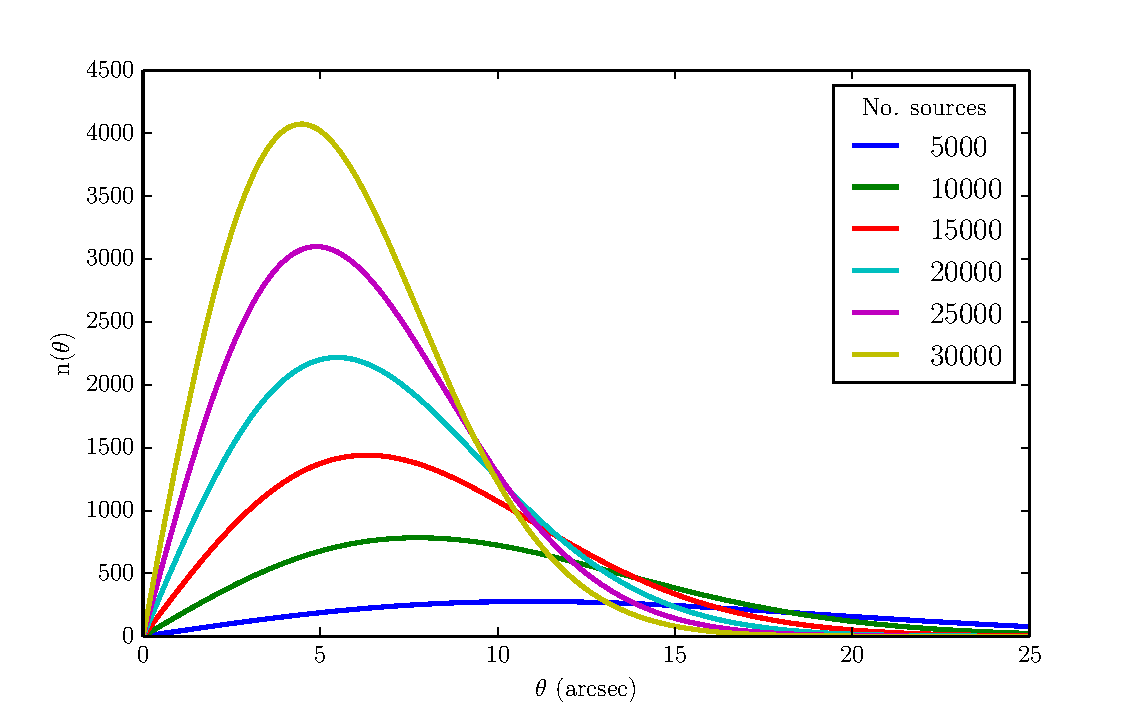
\includegraphics[width=1\linewidth]{figures/theoretical_neighbours.pdf} 
\caption{\footnotesize Theoretical distribution (see Equation  \ref{eq:theoretical_neighbours}) of nearest neighbour distances for an area with the effective area of a WFC image, for fields containing varying numbers of sources.}
\label{fig:theoretical_neighbours}
\end{center}
\end{figure}

% Fig. \ref{fig:theoretical_neighbours} shows this distribution for an area with
% the effective area of the WFC field of view (0.29 sq. deg.) containing varying
% numbers of sources. It can be seen that increasing the density of sources
% increases the number of nearest neighbours at small separations, while
% suppressing the number at greater separations. This has the effect of decreasing
% the peak separation value, $\theta_{max}$.

% This distribution holds for a population of sources randomly distributed
% regardless of brightness. In practice, where the distribution of source
% brightnesses is described by a power law, the susceptibility of a source to
% confusion increases with decreasing brightness; a limiting faint magnitude must
% be chosen in order to define a meaningful confusion rate. For this reason, the
% treatment of nearest neighbour distances adopted in this discussion excludes
% sources fainter than 19th magnitude - i.e. $\rho$ is in fact
% $\rho(\mathrm{m}_0)$, the density of sources down to this faint limit. This
% eliminates the complexity that would be introduced by comparing confusion of all
% sources across fields with different depths.

In order to reproduce the theoretical distribution (Eqn. \ref{eq:theoretical_neighbours}), all sources in 
the area $\Omega$ would need to be recovered. This will never be the case in dense fields, which will modify the 
observed distribution in the sense that the smallest separations will be under-reported - appearing to relatively
boost the proportion of nearest neighbours at larger values of $\theta$.

\begin{figure*}
\begin{center}
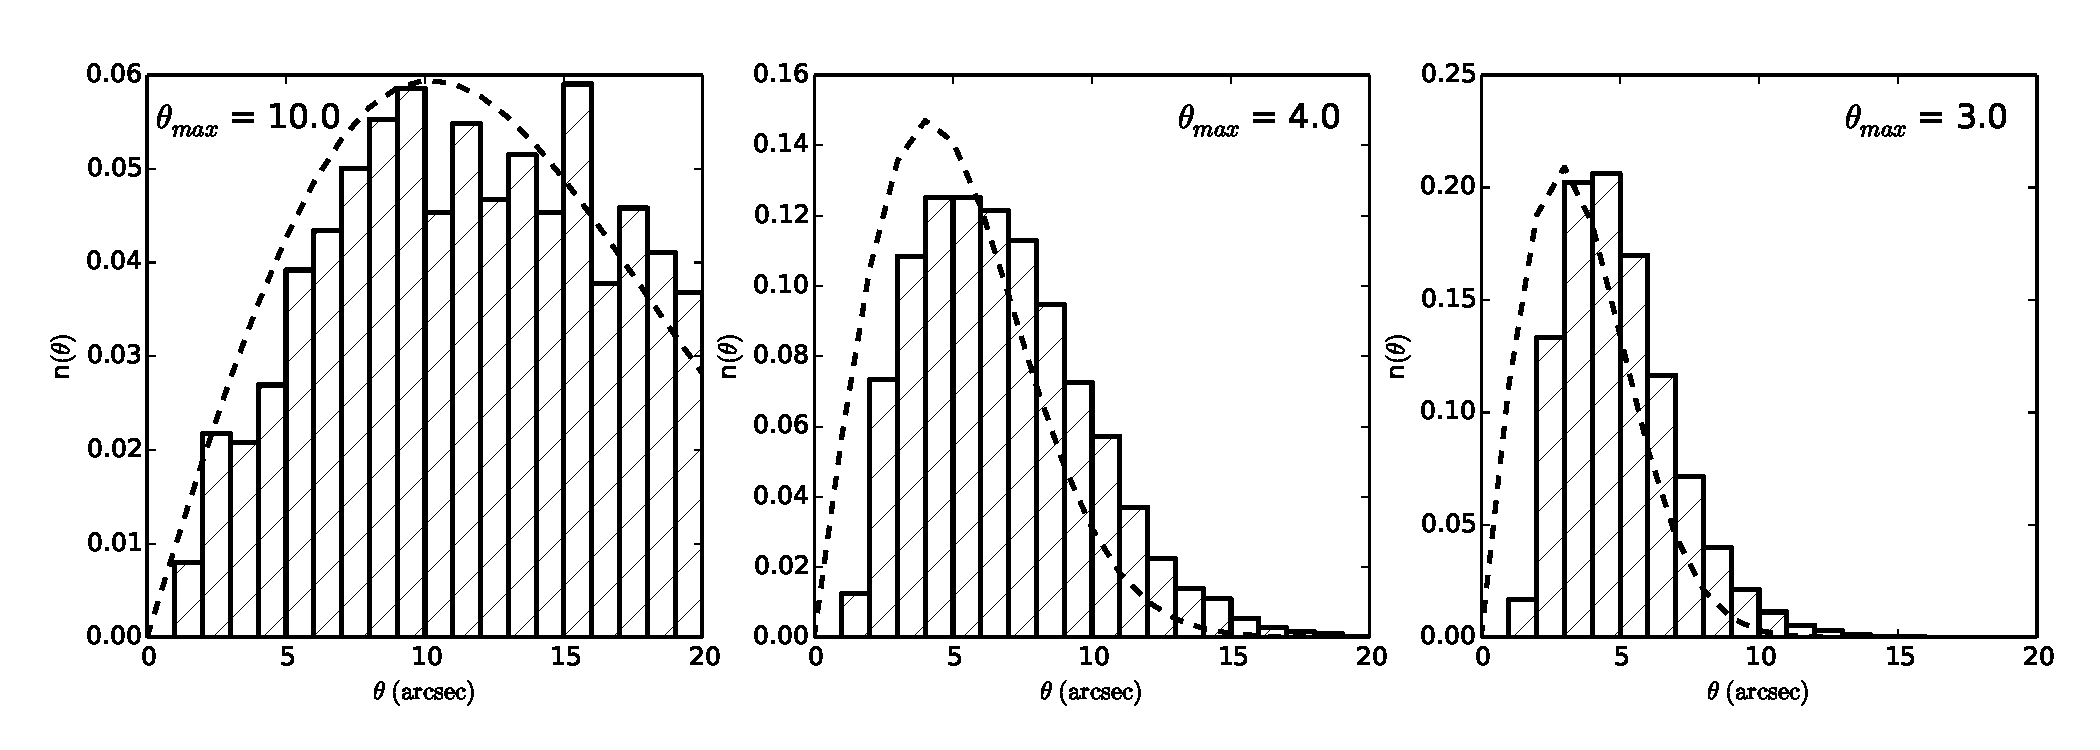
\includegraphics[width=1\textwidth]{figures/neighbours_aquila.pdf} 
\caption{\footnotesize Nearest neighbour distributions for three IPHAS fields, 
normalised to allow the overplotting of theoretical distribution (dashed line).
 Density of fields increase from left to right.}
\label{fig:iphasfield_neighbours}
\end{center}
\end{figure*}

Three test cases are shown in Fig. \ref{fig:iphasfield_neighbours}: these
IPHAS fields, located around $\ell\sim32^{\circ}$, were chosen because they lie in a
region of the survey containing fields spanning a wide range of densities. The
$n(\theta)$ distributions were generated by selecting subregions of the CCDs
such that a border of width 30$^{\prime\prime}$ was excluded, and the nearest
neighbour was identified for each of the sources in the central subregion. This
approach avoids the case where sources close to CCD edges have
their nearest neighbour assigned to a source in the CCD area, when in fact its
nearest neighbour on the sky is located beyond the detector edge. When identifying 
the nearest neighbours for each source in the central region, the 
border region was searched as well.

The fields are displayed in order of increasing density. The left-most field,
4198\_jul2004, contains 3,966 sources - a number sufficiently low that confusion would 
not be expected to make a significant contribution to incompleteness. Fields 
4450o\_jul2009 and 4285\_jun2004, containing 24,291 and 49,150 sources respectively, 
suffer from increasing levels of confusion. The overplotted theoretical distribution 
gives an idea of the amount of confusion; at low field densities, the empirical and 
theoretical distributions agree quite well, while at higher densities the theoretical 
distributions clearly predict closer nearest neighbours than measured.

While the observed nearest neighbour distribution is affected significantly by
confusion most significantly at smaller ($\lesssim10^{\prime\prime}$) separations, the 
observed number of nearest neighbours at larger separations will be less affected. 
Hence, the theoretical distribution best fitting the tail at large $\theta$ values comes 
close to describing the field as if confusion were not an issue.  We have exploited
this property as a means to gauge confusion loss at small separations.  We have fitted
distributions generated from Eqn. \ref{eq:theoretical_neighbours} to the observed 
distributions at $>10^{\prime\prime}$ separation, varying $\rho$ such that the number of 
sources in a field ranged from half to twice its observed value. By calculating $\chi^2$ 
for each fit at large separations, the best fitting value of $\rho$ was found for each, 
identifying the correction that should be applied for confusion.

\begin{figure}
\begin{center}
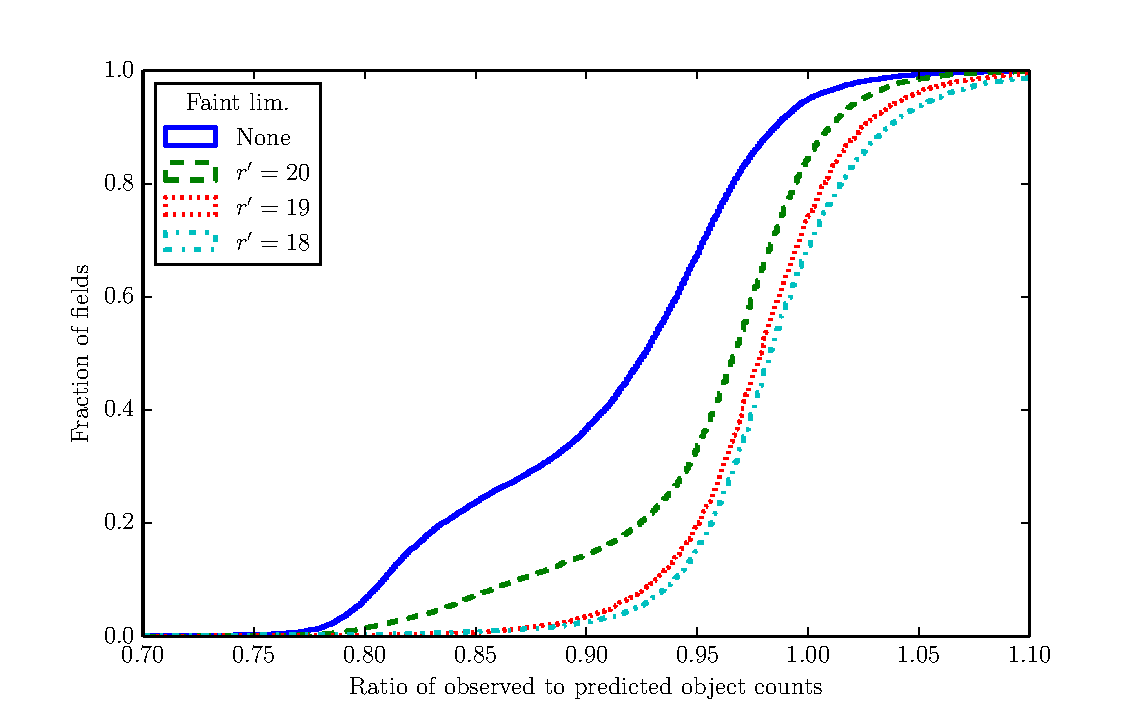
\includegraphics[width=1\linewidth]{figures/confusion_completeness.pdf} 
\caption{\footnotesize Cumulative histogram of $\dfrac{observed}{predicted}$ 
source counts, where the predicted counts were estimated by fitting Equation 
\ref{eq:theoretical_neighbours} to the tail of the nearest neighbour 
distribution. The four curves represent the ratio as determined for sources 
down to three different limiting magnitudes, and an instance where no limit 
was placed on the magnitude of sources.}
\label{fig:confusion_completeness}
\end{center}
\end{figure}

Fig. \ref{fig:confusion_completeness} shows the effect of confusion on the
survey as a whole. Best fitting n$(\theta)$ distribution (corresponding to a
theoretical unconfused source count) was obtained for each IPHAS field, allowing a 
picture to be built up of the impact of confusion. The statistic chosen to 
represent the magnitude of the correction is the ratio of $\frac{observed}{predicted}$ 
sources, where the ``predicted" source count is the count corresponding to the 
best fit theoretical n$(\theta)$ distribution. In order to understand the variation 
in confusion at different limiting magnitudes $m_0$, fits were performed on sources 
brighter than respectively 18th, 19th and 20th magnitudes in $r^{\prime}$, in addition 
to fits across all sources.

In a perfect survey capable of deblending overlapping sources, all fields would
exhibit zero confusion, with their curves jumping from zero to 100\% of all
fields at a ratio of 1.0. In reality some sources will always be lost to
confusion, with the impact increasing the higher the density of objects. Fainter 
objects suffer more from confusion losses as their PSFs are more likely to be 
lost in the vicinity of brighter sources, in addition to their intrinsically higher 
densities (see Fig. \ref{fig:magnitude_turnovers} for examples of the magnitude distributions 
of IPHAS fields). Fig. \ref{fig:confusion_completeness} demonstrates this behaviour as the 
incompleteness takes hold for a greater number of fields as the cut-off magnitude $m_0$ 
is increased.

For a fraction of fields at all values of $m_0$, the best fit to their nearest
neighbour distributions indicates a lower predicted number of sources than
is actually observed. Indeed the median completeness at brighter $m_0$ shows signs of
converging to 0.98--0.99. However, we notice that the maximum ratio returned is $\sim$1.1, 
for fields which lie in regions of lowest density in the map of the Plane. These fields 
would be expected to return a corresponding best fit ratio of 1.0, suggesting that the 
fitting to the n$(\theta)$ distribution tails has an associated uncertainty of $\sim$10\%; 
so large an uncertainty indicates that this method for correcting source counts is not 
sufficiently exact to adopt it for application across the survey.  

Nevertheless, Fig.~\ref{fig:confusion_completeness} can be regarded as a demonstration that, 
as a general rule, at $r < 18$ the impact of confusion in IPHAS is small while (as might be 
expected) it is close to ubiquitous at $r > 20$.  Source counts in the $i$ band are 
higher thanks to the lower extinction -- the same plot for this band shows that 
confusion becomes a minor consideration at $i < ????$ (A NUMBER, PLEASE, HYWEL)

\subsection{Other approximate measures of completeness}
\label{subsec:turnovers} 


There exists a formalism for correcting for the number of sources lost to 
confusion, based upon Eqn. \ref{eq:theoretical_neighbours}, given by
\begin{equation}
\rho = - \rho^{\prime}\frac{\log\left(1-4\rho^{\prime}\pi\theta_{FWHM}^2\right)}{4\pi\theta_{FWHM}^2}
\label{eq:irwin_confusion}
\end{equation}
\noindent where $\rho$ is the actual source density, $\rho^{\prime}$ is the observed density, and $\theta_{FWHM}^2$ 
is the seeing in which the field was observed. The expression was derived in \cite{Irwin1984}, and it was used to correct 
the observed n$(\theta)$ distributions directly in \citet{Gonzalez-Solares2008}. Clearly fields with poorer seeing and 
higher densities will be subject to larger corrections; \citep{Gonzalez-Solares2008} reported that the IPHAS 
Initial Data Release fields suffering from greatest confusion were missing 41\% of their sources.

\begin{figure}
\begin{center}
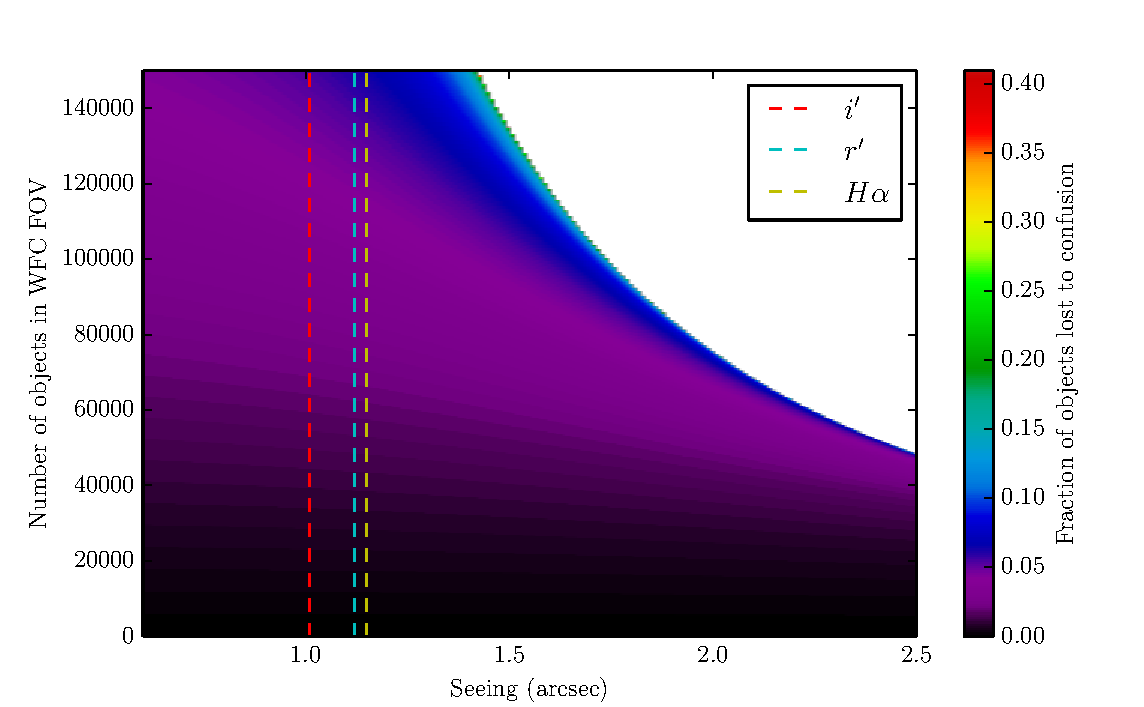
\includegraphics[width=1\linewidth]{figures/neighbour_breakdown.pdf} 
\caption{\footnotesize Correction term in Eqn. \ref{eq:irwin_confusion} for the range of $n_{src} = \rho^{\prime} \times \Omega_{WFC}$ and $\theta_{FWHM}$. Median seeings for each filter are marked by vertical lines. White region denotes domain where Equation \ref{eq:neighbour_breakdown} is true and Equation \ref{eq:irwin_confusion} breaks down.}
\label{fig:neighbour_breakdown}
\end{center}
\end{figure}

However Eqn. \ref{eq:irwin_confusion} does not hold for for the entire
[$\rho^{\prime}$, $\theta_{FWHM}$] space covered by all IPHAS DR2 fields - it
breaks down in dense fields, where the seeing is worse than the median. Fig.
\ref{fig:neighbour_breakdown} shows the variation of the correction term for the range of parameters relevant
to DR2. The white region shows the parameter space in which Eqn. \ref{eq:irwin_confusion} is not 
applicable, where
\begin{equation}
4\pi\rho\theta^{2} > 1
\label{eq:neighbour_breakdown}
\end{equation}
Although this condition is not met so often, the fact that it is some of the time means that its deployment 
eqn.~\ref{eqn:irwin_confusion } across the survey is not viable. 

An approach used in several previous
surveys \citep{Ruphy1997, Cambresy2002, Lucas2008} is to estimate the
completeness limit by taking the magnitude distribution of sources and
identifying at which magnitude the distribution begins to drop off.

As part of a study of stellar populations in the Galactic Plane,
\citet{Ruphy1997} commented on the need for simulated images for a quantitative
study of completeness in their frames, although they opted instead to report a
completeness limit derived from the star count histograms of uncrowded fields.
This approach may serve well in studies of limited sky regions, or if sources
fainter than this putative completeness limit can be excluded without causing
problems. \citet{Ruphy1997} mentioned that confusion due to crowding was the
only source of incompleteness for which they account, choosing to ignore the
``slight variations due to the observing conditions" (an approach unfeasible for
IPHAS).

\citet{Cambresy2002} estimated their completeness from the turnover of 2MASS
magnitude distributions, and reason that their density maps would show imprints
of individual observations had they overestimated their limiting magnitudes.
This would certainly be the case for IPHAS - without any magnitude cut in
place, the field-to-field variation of densities is extremely obvious.  In applying a 
similar treatment of incompleteness, \citet{Lucas2008} quote the 90\% completeness 
limit of the UKIDSS Galactic Plane Survey, noing that in uncrowded fields the modal
depths vary by 0.25 mag due to observing conditions. This method still depends
heavily on the turnover in the magnitude distribution, and relies on 
``visually extrapolating" the histogram.

A single completeness statistic as provided by \citet{Lucas2008} could be used
to apply a uniform completeness correction, although this assumes that all
fields in a survey suffer from the same pattern of incompleteness. Even if this
were indeed the case, only the count of sources brighter than the given
completeness limit could be corrected; it is not possible with this information
to correct the count going deeper.

\begin{figure*}
\begin{center}
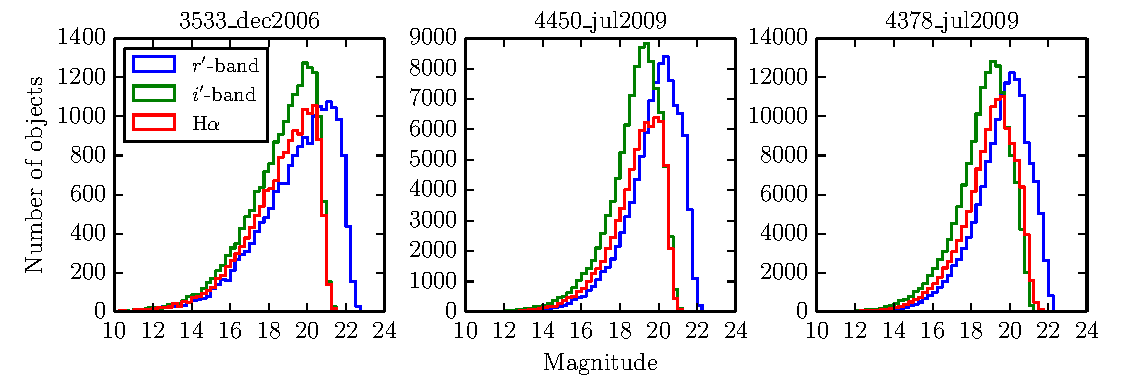
\includegraphics[width=1\textwidth]{figures/magnitude_turnovers.pdf} 
\caption{\footnotesize Magnitude distributions for three IPHAS fields of 
increasing density. From left to right, fields have $r^{\prime}$-band source 
counts of 18,113, 99,061 and 153,430. A requirement that sources counted here 
have $nBands>1$ places the greatest constraint on $i^{\prime}$-band counts, 
as redder sources are picked up in the $i^{\prime}$-band only.}
\label{fig:magnitude_turnovers}
\end{center}
\end{figure*}

Fig. \ref{fig:magnitude_turnovers} shows the magnitude distributions for three IPHAS fields. 
A visual inspection would suggest that incompleteness sets in at $\sim$20th mag or fainter in
$r$ and at $\sim$19th in $i$ and $H\alpha$. Attempts to automate the determination of turnover 
magnitude for all fields are hampered by the facts that the mode of these distributions are 
dependent on the chosen binning, and that the magnitude distributions of many fields plateau 
before dropping off.  But it is already clear from the previous section and 
Fig.~\ref{fig:confusion_completeness} that the full picture is more complicated, with some small 
residual source loss still affecting magnitudes as bright as 18 to 19. In short, there is good reason 
to address correction rigorously on a field by field basis. 


\subsection{Artifical source injection}  
A thorough treatment of incompleteness in any survey requires measuring its
sensitivity to sources over the entire magnitude range of interest - this is best achieved 
by simulating observations and then processing these simulated frames in the same way as 
the original data. This method (in addition to the magnitude distribution method 
discussed in $\S$\ref{subsec:turnovers}) was used and described by \citet{Harvey2006} as part 
of a study of interstellar clouds observed by Spitzer.

Such an approach is much more powerful, as statistics can be returned on
magnitude bins, rather than on the entire magnitude distribution down to a
specified faint limit. This requires the simulation of sources of all
magnitudes, resembling the real data as closely as possible, without being too
costly to generate in either computing power or time.

For the purposes of correcting the density map, the completeness of each field
was assessed using the images and catalogues of CCD 4 only. Using only one of
the WFC CCDs per field cuts the processing time by a factor of four, bringing
the total time necessary to compute the completeness of the entire survey down
to a little over one week (using a high-performance multi-node cluster). Due to the 
fact that DR2 preferentially selects sources from the centre of fields (closer to the 
optical axis), CCD 4 -- the most central of the mosaic -- was selected as the chip 
to represent each field (see $\S$\ref{subsec:completeness_ccd4} for further discussion).

The main steps of the completeness calculation were as follows. First the
typical properties of an image were determined, and used to generate synthetic
sources that closely resemble genuine stellar sources (Section \ref{subsec:artificial_sources}). 
The parameters of these synthetic sources were recorded and then catalogues were generated, via 
the pipeline software, from the new frames with the added synthetic objects. The tables of 
synthetic source parameters were cross-matched against the newly generated catalogues, and the 
rate of recovery was measured (Section \ref{subsec:recovery}). The fraction recovered at 
different magnitudes will allow a completeness curve to be built up for each field, and 
uniformly computed corrections can then be applied across the entire survey.

\subsection{Simulating stellar sources}
\label{subsec:artificial_sources}
The complexity of simulating stellar sources depends on the accuracy with which
the real sources are to be recreated. A first order approximation might be a
circular PSF characterized by a two-dimensional Gaussian, requiring only three
parameters - FWHM, peak height and centroid coordinates. A cursory glance at the reduced IPHAS frames reveals that a 
perfectly circular PSF will not yield realistic stellar sources - a more complex approximation is needed 
(see Fig. \ref{fig:fitting_profiles}).

\begin{figure}
\begin{center}
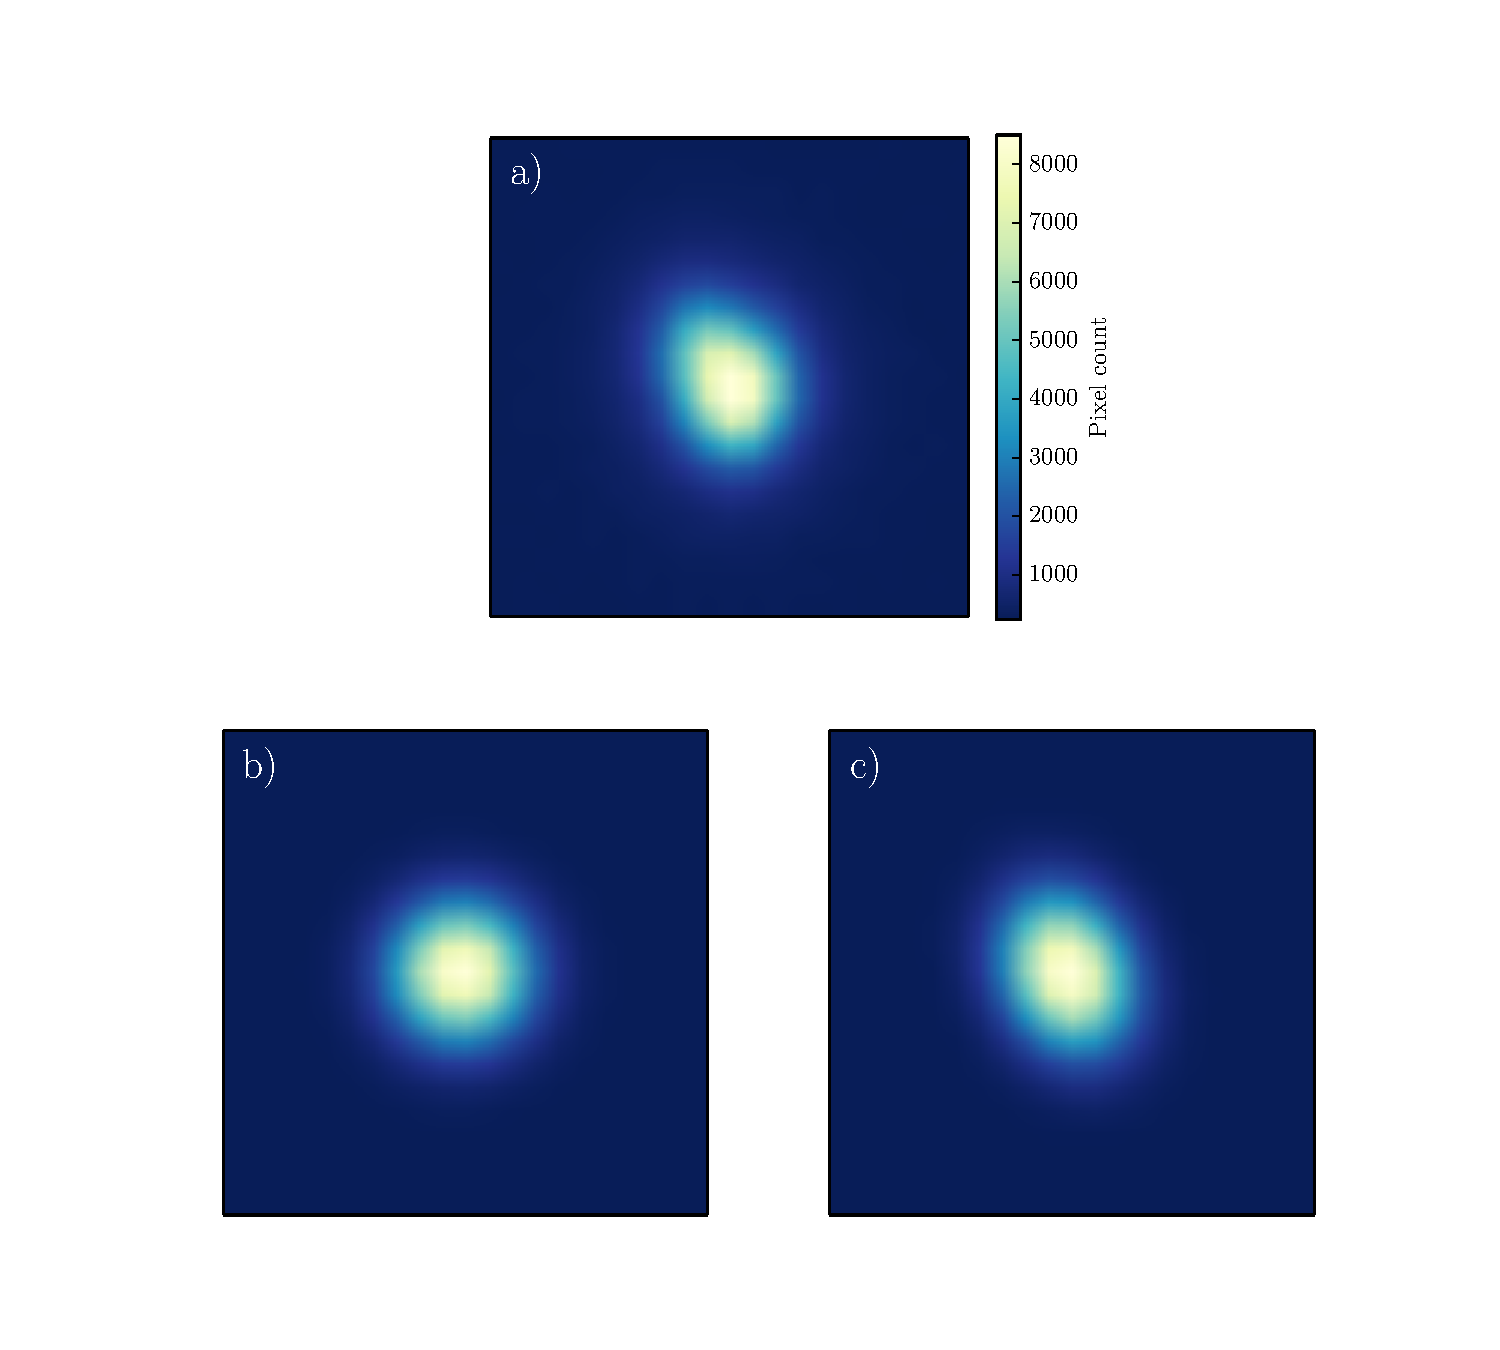
\includegraphics[width=1.0\linewidth]{figures/fitting_profiles.pdf} 
\caption{\footnotesize \textbf{a)} 16th magnitude source from an IPHAS field. 
\textbf{b)} Simulated source generated using best-fit parameters of a 2D 
circular Gaussian. \textbf{c)} source generated using best-fit parameters of 
a 2D elliptical Gaussian.}
\label{fig:fitting_profiles}
\end{center}
\end{figure}

The parameters returned by the aperture photometry performed on the DR2 images indicate the following 
should be included to accurately recreate a stellar source:
\begin{itemize}\itemsep
\item Flux
\item FWHM
\item Ellipticity
\item Position angle
\item Sky background level
\item Coordinates (or pixel position on detector).
\end{itemize}
\noindent The choice of each is described below.

\subsubsection{Flux}
\label{subsubsec:flux}
The relation between total flux and magnitude was determined per field by fitting a power law to the photometry returned 
by \textsc{imcore}.

\textit{Mention that flux height is initially used? It doesn't have to be, and if code is rewritten for publication this 
step could be removed.  JED - if of no material significance, can be left out.  I assume we are later..}

In order to insert a source of a given magnitude $m_0$, it is necessary to understand what flux in counts per unit time
that source should have. The magnitude of an object is determined by
\begin{equation}
m = ZP - 2.5 \times \log_{10} {\dfrac{c}{t}} - APCOR - PERCORR
\label{eq:aperture_photometry}
\end{equation}
\noindent where $ZP$ is the photometric zeropoint of the image as determined via the DR2 uniform calibration \citep{ }, $c$ 
is the measured counts within the defined aperture, $t$ is exposure time in seconds, while $APCOR$ and $PERCORR$ are small 
correction terms. $APCOR$ is an aperture correction term calculated by the pipeline software, \textsc{imcore}, which uses 
the curve-of-growth of stellar sources to determine the correction required to transform the chosen aperture measurement to 
total flux (suitable reference). $PERCORR$ is a sky calibration correction, obtained by comparing dark sky regions with the 
median across each CCD. $ZP$, $APCOR$ and $PERCORR$ are all taken from the pre-existing catalogue headers.

\subsubsection{PSF shape parameters: Full-width at half-maximum and ellipticity}
\label{subsubsec:parameter_fwhm}

Initially the parameters of genuine sources in IPHAS frames were determined by
fitting elliptical two-dimensional Gaussian profiles to each source detected by
\textsc{imcore}, building up lists of best fit parameters for the purpose of
generating realistic artificial sources.  Parameters of sources were excluded from 
these lists if they exhibited one of the following behaviours: 
\begin{itemize}\itemsep \item The source position returned is
further than 5 pixels from the position reported by \textsc{imcore} \\- these
fits are likely to have been disturbed by nearby sources \item The
peak value of the best-fit Gaussian is $>55000$ counts \\- this is the regime
for the WFC where bright sources saturate, distorting the PSF. \item The
position angle is measured to be exactly zero \\- in these cases the fit is
assumed to have failed {\bf or the measured PSF is indistinguishable from 
circular (JED comment)??}\end{itemize}

The best fit full-width half maximum (FWHM) values returned for the semi-major and 
semi-minor axes of the sources were gathered for each of the fields entering this 
exploration, and Gaussians were then fit to the distribution to recover the distribution
mean and $\sigma$. 
%Fig.
%\ref{fig:parameter_fwhm} shows the distributions for four IPHAS fields, in
%addition to the central positions of the best fit Gaussians.

%\begin{figure} 
%\begin{center}
%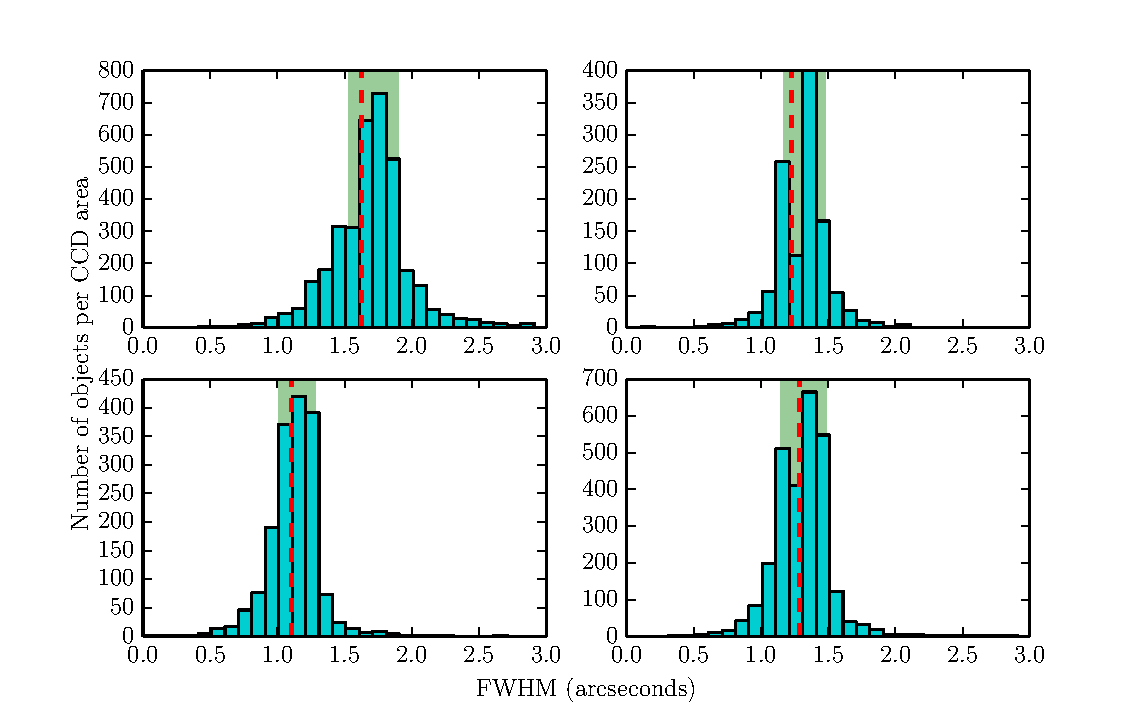
\includegraphics[width=1.0\linewidth]{figures/parameter_fwhm.pdf}
%\caption{\footnotesize Distribution of best fitting FWHM values in arcseconds for sources from four randomly selected IPHAS DR2 fields. Values were obtained by fitting elliptical Gaussians to every stellar source in CCD4 of the IPHAS
%field. FWHM values reported here are for the Gaussian profile along the semi-
%major axes of the sources. \textbf{Red lines} denote the median FWHM as
%determined by \textsc{imcore} for CCD4. \textbf{Green shaded areas} highlight the regions centred on the best fit FWHM 
%for the distributions, and encompass the area $\pm\sigma$.} 
%\label{fig:parameter_fwhm} 
%\end{center} 
%\end{figure}

This exercise quickly revealed that the median(???) FWHM values obtained in this way
were in good agreement with those determined by \textsc{imcore}, confirming that the pipeline-specified 
value can be re-used safely for articial source generation. 
%Fig. \ref{fig:parameter_fwhm} shows how the median FWHM values fall within 1$\sigma$ of the best fit Gaussian distributions for four randomly
%selected IPHAS DR2 fields.

%\subsubsection{Ellipticity}
%\label{subsubsec:ellipticity}
%\begin{figure} 
%\begin{center}
%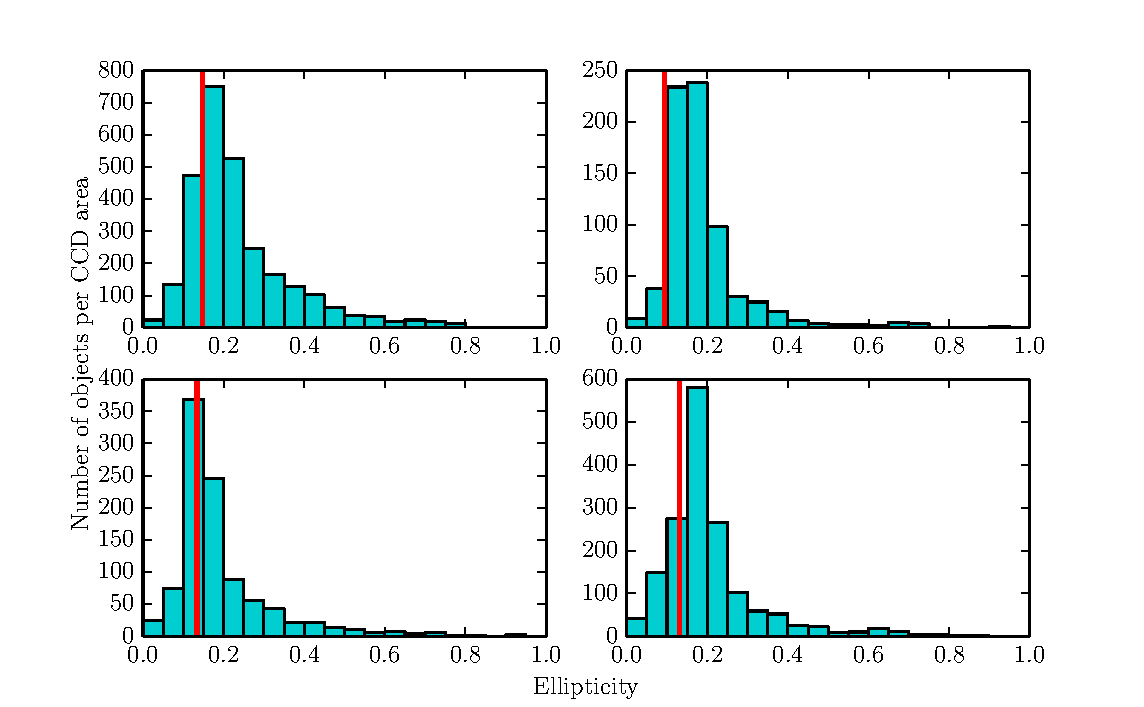
\includegraphics[width=1.0\linewidth]{figures/parameter_ell.pdf}
%\caption{\footnotesize Distribution of ellipticities for all stellar sources in
%four randomly selected IPHAS fields. Ellipticities were computed from the
%profiles of the elliptical Gaussians best fitting each object along their semi-
%major and -minor axes. \textbf{Red lines} denote the median ellipticities for
%CCD4 of each field as determined by \textsc{imcore.}} 
%\label{fig:parameter_ell}
%\end{center} 
&\end{figure}

The treatment of ellipticity followed that of FWHM values -- constructing a reliable measure of field-wide ellipticity  
from the median of the best-fit FWHM values across the field and the relation
\begin{equation}
e=1-\frac{\mathrm{FWHM}_{min}}{\mathrm{FWHM}_{maj}}
\label{eq:ellipticity}
\end{equation}
\noindent (where FWHM$_{min}$ and FWHM$_{maj}$ are the full-width half-maxima along sources' semi-minor and semi-major 
axes respectively).  In similar vein, comparisons with ellipticities returned by the pipeline indicated that these too 
were in good enough agreement to give confidence that they coud be re-used in artificial source generation.

%Fig. \ref{fig:parameter_ell} shows the distributions of ellipticities as
%determined by Equation \ref{eq:ellipticity} and the FWHM values determined in
%Section \ref{subsubsec:parameter_fwhm}. The median ellipticity value as
%determined by \textsc{imcore} is denoted by a red line. It can be seen that the
%median values for three of the four test fields are slightly optimistic (i.e.
%underestimate the ellipticities measured from 2D Gaussian fits). Owing to the
%fact fields displaying ellipticities greater than 0.3 were excluded from release 
%in DR2, the slight mismatch between the median of the fitted ellipticities and the 
%comparatively optimistic median calculated by \textsc{imcore} will never be so large 
%that it will significantly affect the recovery of sources.

%\textit{Seems a bit weak. But returned magnitude shouldn't really be affected by 
%ellipticity - we're not PSF fitting each source. Position might be affected, but only by 
%a very small amount.  JED - it is actually all rather confusing just now... see
%email: the clear up will need to start in the previous sub-section.}

\subsubsection{Position angle}
\label{subsubsec:position_angle}
%Conclusion in thesis is that most fields' PA distributiuons are too flat (or
%at least not nicely Gaussian) to confidently obtain a PA, so it's dropped. Is
%such a subsection even worth including here?
The typical distribution of position angle (PA) within a field is quite broad and non-Gaussian in
appearance.  In practice, there is no reason to expect the choice of PA to significantly influence 
the ability to recover an artificial source -- hence it is set at {\bf Hywel - just state what you 
did -- is it always set equal to zero, or what?}

\subsubsection{Position}
\label{subsubsec:position}
Object $x$ and $y$ pixel positions were drawn randomly from uniform
distributions across the 2048$\times$4096 pixels of the WFC CCDs.

The completeness calculated for the unvignetted CCD 4 of each field was taken to represent 
the completeness over all four CCDs.  This allowed the border zone -- which can complicate the 
appraisal of completeness -- to be easily defined: a rectilinear zone 10 arcsec (or 30 pixels) wide
inside the CCD edges was imposed such that no artificial source could be placed within it.  
\textsl{Include plot of used region of all 4 CCDs here or in map generation section ...JED - 
in the map generation section}.  This made sure that no injected artificial source would lose
flux across the CCD edge.


\subsection{Practical implementation of artificial source injection}

Ideally measuring the completeness using artificial sources would be done by adding a single source 
at a time, verifying whether or not it is detected. This process would be repeated as many times as required 
to obtain decent statistics, for the entire magnitude range of interest. This would be the route taken in the 
absence of any limitations on either time or computing resources.   The limiting factor in this 
is the computing time taken for the basic step of catalogue generation (20 sec in this case).  To generate the 
number of sources detailed in Table \ref{table:number_artificial} $\sim$ 65 hours would be required to process 
just one field.

To reduce the cost, multiple sources needed to be inserted into each image simultaneously. It was necessary to 
ensure that not too many sources were inserted at any one time; inserting too high a number would modify the intrinsic 
properties of the image - for example, probing the completeness of an originally sparse image with a high number of 
artificial sources inserted would not return statistics useful for understanding the original image. The value of 
$\frac{\delta n}{n_{image}}$ needed to be kept sufficiently low, where $\delta n$ is the number of artificial sources 
added to the image, and $n_{image}$ is the number of sources present originally. The quality control 
information available for DR2 fields report that the most sparsely populated fields contain more than 1000 stars. This 
is not an extremely constraining limit; a maximum of up to 50 stars was chosen as a value that would keep 
$\frac{\delta n}{n_{image}}$ below 0.05 for all fields.   Allowing up to 50 sources per artificial source injection 
increases processing efficiency, but the low value of $\frac{\delta n}{n_{image}}$ is too little to sample the 
pre-existing magnitude distribution of the sources in each image faithfully.  Hence, the approach adopted was to 
split the magnitude range of interest into bins $0.25$ mag wide, inserting sources from only one bin at a time in each 
catalogue regeneration.

\begin{table}
\begin{center}
\begin{tabular}{|c|c|c|c|c|}
\hline
\multicolumn{2}{|c|}{Magnitude bin} & & & \\ \hline
Start & End & $N$ & $M$ & $No.\ sources$ \\ \hline
12.0 & 12.25 & 10 & 10 & 100 \\
12.25 & 12.5 & 10 & 10 & 100 \\[-1.5mm]
\vdots & \vdots & 10 & 10 & 100 \\
14.5 & 14.75 & 10 & 10 & 100 \\
14.75 & 15.0 & 10 & 10 & 100 \\ 
15.0 & 15.25 & 20 & 10 & 200 \\[-1.5mm]
\vdots & \vdots & 20 & 10 & 200 \\
16.25 & 16.5 & 20 & 10 & 200 \\
16.5 & 16.75 & 30 & 10 & 300 \\[-1.5mm]
\vdots & \vdots & 30 & 10 & 300 \\
17.75 & 18.0 & 30 & 10 & 300 \\
18.0 & 18.25 & 40 & 10 & 400 \\[-1.5mm]
\vdots & \vdots & 40 & 10 & 400 \\
18.75 & 19.0 & 40 & 10 & 400 \\
19.0 & 19.25 & 50 & 10 & 500 \\
19.25 & 19.5 & 50 & 10 & 500 \\
19.5 & 19.75 & 50 & 15 & 750 \\
19.75 & 20.0 & 50 & 15 & 750 \\
20.0 & 20.25 & 50 & 20 & 1000 \\[-1.5mm]
\vdots & \vdots & 50 & 20 & 1000 \\
20.75 & 21.0 & 50 & 20 & 1000 \\\hline
\multicolumn{3}{|r|}{Total:} & 410 & 12300 \\\hline
\end{tabular}
\caption{\footnotesize Number of artificial sources added per magnitude bin. $No.\ sources$ denotes total number that will be generated over $M$ runs. $N$ is the number of sources that will be added to each image, which will be repeated $M$ times. A total of 123000 are added per field, across 410 images containing artificial sources.}
\label{table:number_artificial}
\end{center}
\end{table}

Table \ref{table:number_artificial} details $N$, the number of sources inserted per image, and $M$, the number 
of artificial images generated for reprocessing and recovery for each magnitude bin. $N$ rises  
with increasing magnitude and is capped at 50 at the faint end for the reasons discussed above. To accumulate a 
larger number of sources injected in the faintest bins, and minimize noise where the most significant corrections 
arise, $M$ increases from 10 to 15 at $m_0 = 19.5$, and then to 20 at $m_0 = 20.0$.  This setup requires around 
2.2 hours ($\sim$20 s $\times$ 410 \textsc{imcore} runs). For the 14,115 fields that make up DR2, this results in 
a total computing time of $\sim$31000 hours. Utilizing 128 CPUs simultaneously brings the total time to estimate 
completeness for the entire survey in a single band to $\sim$10 days.

\subsection{Recovery of simulated sources}
\label{subsec:recovery}

Cross-matching the recovered sources to the added artificial sources required the imposing of matching thresholds 
in both position and brightness. While ideally a recovered source should lie centred on the exact $x$,$y$ pixel 
position where it was added, there is no guarantee that \textsc{imcore} will report unchanged centroid coordinates. 
Background variations in the original image, pixel binning and blending may cause the reported centroid to shift 
by a small amount: hence, a generous upper limit of 5 pixels was set on this shift away from the recorded 
position of inserted sources.  {\bf JED: what was a typical shift?  ...might be worth a mention to reassure the 
reader.} 

Simply cross-referencing the recorded position of an artificial source with the new set of catalogues was not 
sufficient to ensure sucessfully recovery. A constraint on the difference between the recovered magnitude, $m_rec$ 
of the source and its insertion value $m_0$ is needed too, in order to reduce spurious crossmatches between added 
sources and pre-existing nearby sources (typically of different brightness).  Choosing a bound on this offset, 
$\Delta_m = m_{rec} - m_0$, was more involved than for pixel position.  Previous attempts to use artificial photometry 
to understand incompleteness have faced similar issues.  For example, \citet{Mateo1986}, as part of a study of a 
globular cluster in the Large Magellanic Cloud, added artificial stars to images using \textsc{DAOPHOT}: they considered 
a source recovered if it was returned at the same coordinates at a magnitude within 0.5 of the inserted value. 
\citet{Harvey2006} used this approach in a study of stellar sources in the Serpens molecular cloud, and plotted 
the modulus of the average difference for artificial sources injected into their data, finding a range from 
0.1 mag at $\sim$10-13 mag to more than 0.5 mag at $\sim$15 mag.

For each field, the distribution of the modulus of $\Delta_m$ was binned up and the 
modal value determined. For a number of fields, the modal value reached $\approx$0.4
mag - an effect that would require a $\Delta_m$ tolerance of $>$0.5 mag. Such
a large tolerance would likely result in many spurious cross-matches and hence
an unduly optimistic estimate of completeness fractions, especially at fainter
magnitudes.

\begin{figure}
\begin{center}
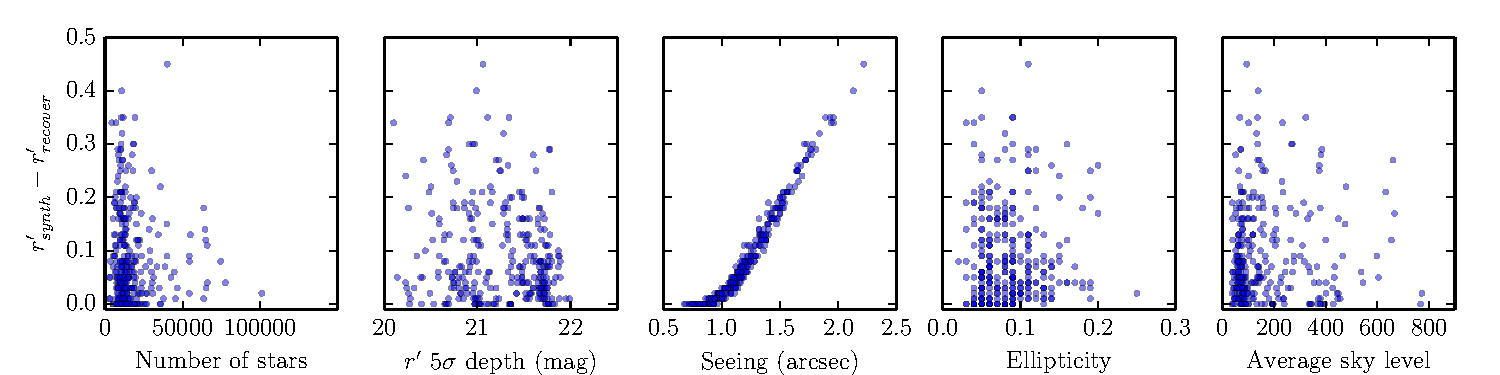
\includegraphics[width=1\linewidth]{figures/magdiff_parameters.pdf} 
\caption{\footnotesize{Modal difference between artificial inserted and
recovered magnitude difference per field, plotted against field
parameters.newline textsl{Redo this plot with only seeing panel. Or could
drop entirely.}}}
\label{fig:magdiff_parameters}
\end{center}
\end{figure}

In the course of investigating whether field conditions correlated with the
offset of the $\Delta_m$ distribution, the modal shift value for each field
was plotted against a number of field parameters. The resulting plots, seen in
Fig. \ref{fig:magdiff_parameters}, clearly show that the modal offset in $\Delta_m$
correlates most strongly with the PSF FWHM (the 'seeing').  The relationship
is such that the returned magnitudes from an image are offset by a uniform amount 
rather than showing increased spread - this lies behind the tightness seen in 
the correlation between $\Delta_m$ values and PSF FWHM, up to the highest
values encountered in the survey. This justified the application of a uniform
shift to all measured {\bf recovered?} magnitudes from an image, applied to bring 
the median $\Delta_m$ of a field to zero.

Having reduced the systematic shifts to $\Delta_m$ values, a bound on the acceptable
corrected difference $\Delta_m$ still needs to be set. As illustrated in 
Fig. \ref{fig:magnitude_match}, the completeness curves
remain relatively unchanged at $r^{\prime}\lesssim19$ as the $\Delta_m$ threshold is
varied between 0.5 and 0.1 mag (the magnitude range of interest for correcting
the density map). A threshold value of 0.25 mag was chosen as a compromise
between avoiding acceptance of a large number of spurious detections at the faint
end of the magnitude distribution, and ensuring that few objects are missed
due to the occasional large $\Delta_m$ value.

{\bf JED: the figure can lose the blue lines, and become a single panel}

\begin{figure}
\begin{center}
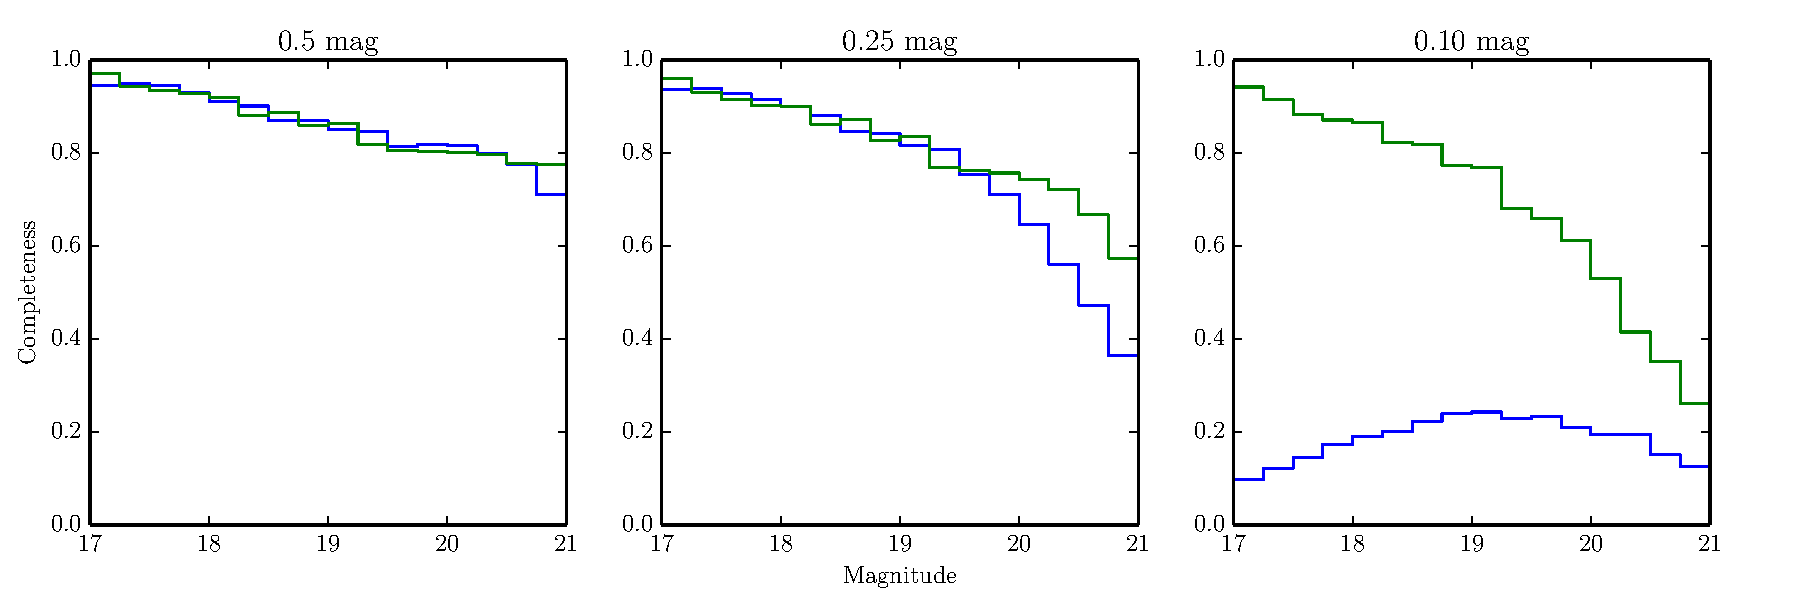
\includegraphics[width=1\linewidth]{figures/magnitude_match.pdf} 
\caption{\footnotesize{$r^{\prime}$-band completeness fractions (\textbf{green}) for IPHAS 
field 4121o\_jul2009, with offset tolerances between inserted and recovered magnitudes of 0.5, 
0.25, and 0.1 mag (from left to right). \textbf{Blue:} Completeness fraction before 
implementing the scaling to total flux vs. magnitude relation (see Section \ref{subsubsec:flux}) 
and the shift to account for the effect of seeing (see Section \ref{subsec:recovery}). 
\textbf{Green:} Completeness fraction after applying these corrections. \newline
\textit{The point of this plot is currently to emphasise the effect of scaling to total flux rather 
than peak height. But if we're not mentioning peak height at all then this plot should be regenerated 
with only the green lines, to show the effect of changing matching tolerance.}}}
\label{fig:magnitude_match}
\end{center}
\end{figure}

\subsection{Completeness fractions}

\begin{figure*}
\begin{center}
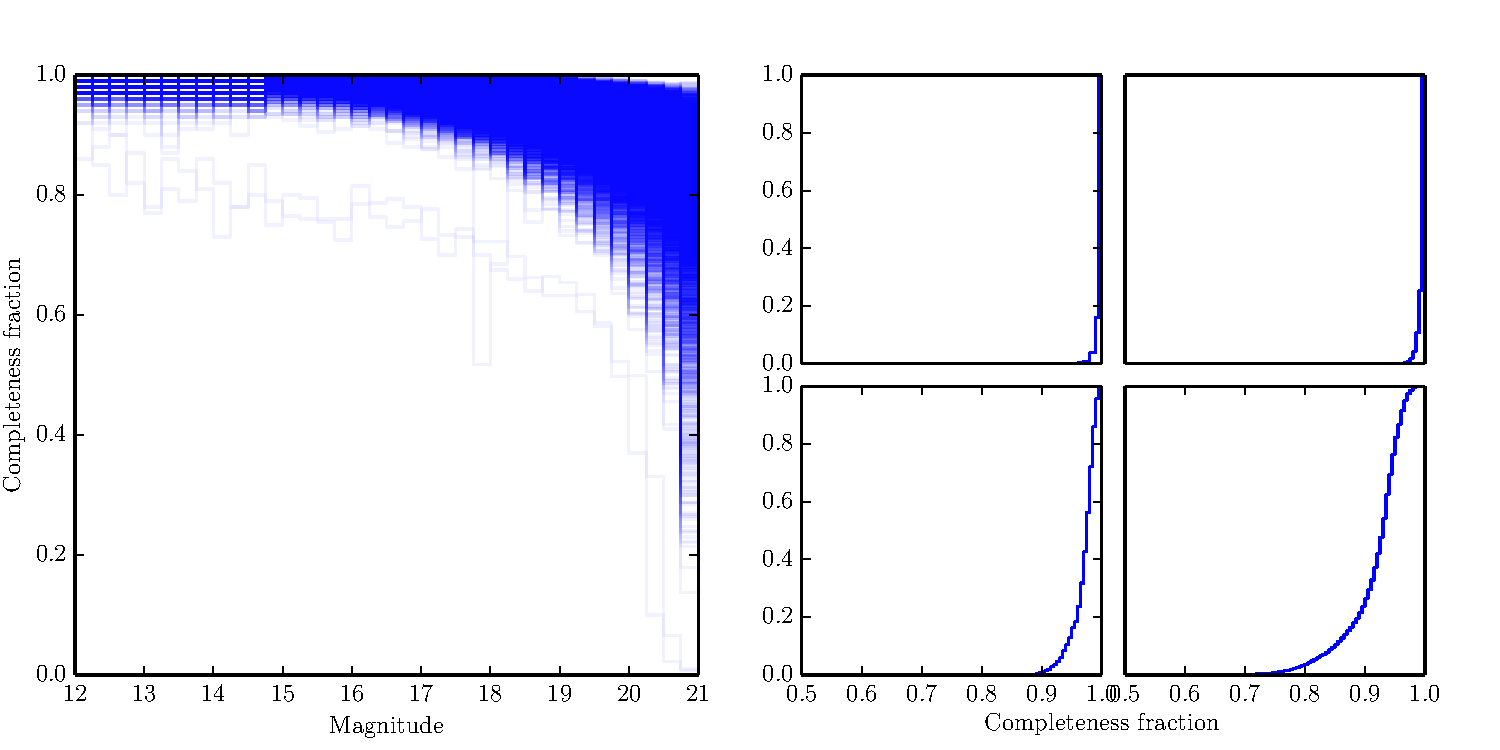
\includegraphics[width=1\textwidth]{figures/completeness_curves.pdf} 
\caption{\footnotesize \textbf{Left:} Plot of every completeness curve in DR2, for magnitude bins of width 0.25 in range $12.0<r^{\prime}<21.0$. \textbf{Right:} Cumulative histograms of field completeness for magnitude bins \textbf{a)} 12.0-12.25, \textbf{b)} 15.0-15.25, \textbf{c)} 18.0-18.25, \textbf{d)} 20.0-20.25.\textit{Regenerate leaving out Capella-afflicted field pais!}}
\label{fig:completeness_curves}
\end{center}
\end{figure*}

Fig. \ref{fig:completeness_curves} shows the completeness curves of all DR2 fields; the discrete quantisation of completeness is more prominent at the bright end due to lower artificial sources being injected to assess the incompleteness of bright sources. The upper two cumulative histograms shown in \ref{fig:completeness_curves} show that incompleteness remains low at bright magnitudes, with a median completeness of 99.5\% at $r^{\prime}$=15. At 18th magnitude the median completeness of IPHAS is 97.7\% complete, falling to a median completeness of 93.1\% at 20th magnitude.

In order to apply completeness corrections when generating the density map, each detected source needs to contribute to the map by a factor that takes into account the incompleteness of sources of similar magnitude from its field of origin. In order to characterise the incompleteness fraction of each field as a quantity varying continuously with magnitude, a function was fit to the measured completeness fractions of each field, of the form
\begin{equation}
C(r^{\prime}) = \alpha - \gamma \times \mathrm{e}^{\frac{r^{\prime}}{\beta}}
\label{eq:completeness_curve}
\end{equation}
\noindent where $\alpha$, $\beta$, and $\gamma$ are parameters allowed to vary to find the best fit for each field. These parameters were collected and formed a lookup table for use in correcting the density map. The curves of this form can be seen plotted for every field in Fig. \ref{fig:completeness_fits}.

\begin{figure}
\begin{center}
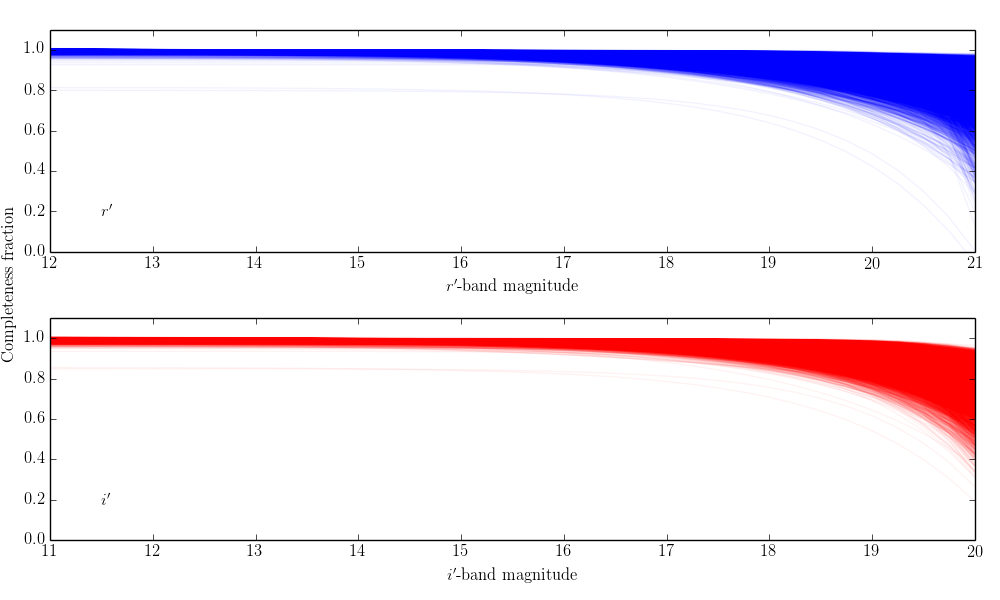
\includegraphics[width=1\linewidth]{figures/completeness_fits2.png} 
\caption{\footnotesize Best fits to completeness curves (as illustrates in Fig. \ref{fig:completeness_curves}) for both $r^{\prime}$ (\textbf{upper}) and $i^{\prime}$ (\textbf{lower}) catalogues.}
\label{fig:completeness_fits}
\end{center}
\end{figure}

As mentioned in Section \ref{subsec:artificial_sources}, the completeness curves generated from CCD 4 of each field were used to represent those of the field as a whole. To ensure that this approach was sensible, a random set of fields had completeness curves generated for all four CCDs in order to compare completeness curves and ensure that the variation between chips was acceptably low. For the magnitude range $12<r^{\prime}<21$, standard deviations in the completeness corrections were calculated. At $r^{\prime}=19$, the deviation in completeness corrections between CCDs reaches as high as 0.025 - these cases occur where a bright star appears in one or more CCD of the field. These cases are rare; the median $\sigma$ at $r^{\prime}=19$ is 0.005.


\section[]{The density maps}
\label{sec:dmap}
\textsl{Cut down contents of Chapter 5, describing how sources are counted, resolutions/limits available.}

\subsection{Source counting}
\label{subsec:counting}
The IPHAS footprint was split into cells of the desired resolution (the final cell size was $1^{\prime}\times1^{\prime}$), and for each cell, a table identifying the extent of every image contributing to DR2 (at the CCD level, i.e. $4~\times$ sub-images distinguished per field) was queried to identify which intersect the cell (either completely or in part). In order to calculate the coverage of each CCD, the pixel coordinates of each corner were determined, with an unusable border region taken into account for each of the four CCDs, in order to exclude sources detected far from the WFC optical axis (source counts from these regions would be unreliable). Fig. \ref{fig:ccd_coverage} shows the extents of the CCDs that were included when calculating coverage.

\begin{figure}
\begin{center}
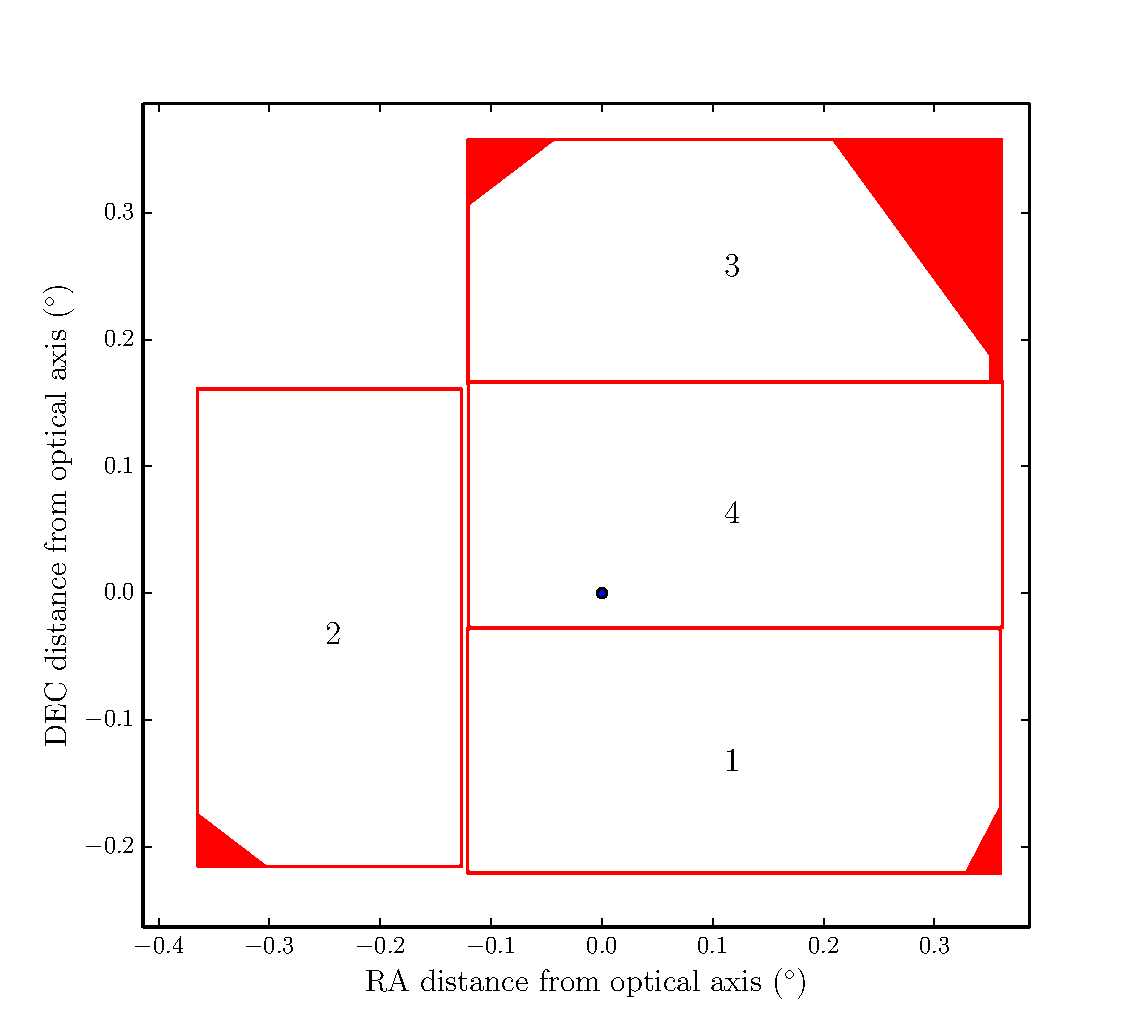
\includegraphics[width=1\linewidth]{figures/ccd_coverage.pdf} 
\caption{\footnotesize Area discarded when calculating coverage of density map cells by IPHAS CCDs contributing to DR2. Blue point denotes optical axis of the WFC. CCD chips are numbered.}
\label{fig:ccd_coverage}
\end{center}
\end{figure}

For each cell, the relevant files identified in by the coverage table was accessed, and all sources within the cell boundaries selected from the intersecting fields. Sources meeting the following criteria were retained:
\begin{itemize} \itemsep
\item Morphology classification -1, -2 or +1
\item Brighter than faint limit (default $r^{\prime}=19$)
\item Flag errBits $<$ 64 for band of interest
\end{itemize}
\noindent where the errBits criterion eliminates sources with bad pixels within their PSF, which are truncated, or which are vignetted. The exclusion zone shown in Fig. \ref{fig:ccd_coverage} will have eliminated the majority of such cases, while this pass removed sources affected by issues such as bad columns and hot pixels.

For each remaining source, a \textit{corrected contribution} to the number count of the cell was computed from the completeness curves generated in Section \ref{subsec:completeness_fractions}. The table containing $\alpha$, $\beta$, and $\gamma$ values (defining Eqn. \ref{eq:completeness_curve}) for each field was read in, the values relevant to the current field identified, and the magnitude of the source under consideration used to calculate the corrected contribution. The original ($\phi$) and corrected ($\Phi$) source counts were recorded, along with the area of the intersection between the cell and the IPHAS field. Each estimate of total cell occupation, $\Phi^{\prime}$ is given by 
\begin{equation}
\Phi^{\prime} = \dfrac{\Phi}{coverage fraction}
\label{eq:corrected_density}
\end{equation}
\noindent and the estimate of uncertainty is simply the Poisson noise of the observed area scaled to the cell:
\begin{equation}
\Phi^{\prime}_{err} = \dfrac{\sqrt{\Phi}}{coverage fraction}.
\label{eq:corrected_poisson}
\end{equation} 
\noindent This is repeated for each CCD covering the cell, and for each cell in the density map.

This method of populating density map cells provides additional information compared to the averaging of repeated sources. At $1^{\prime}\times1^{\prime}$ resolution, the density map contains 6,537,051 cells overlapping with IPHAS photometry. Of these, 92.9\% have an overlap with a second IPHAS CCD, with 38.3\% having a third. These cells provide an estimate of the variance in source counts between observations, which in turn can be compared with the Poisson uncertainty calculated for these cells. \textit{Ref section that contains this discussion.} In cases where multiple CCDs covered the same fraction of a cell, the count from the CCD observed under the best conditions was used to inform the density map.

\subsection{Bright stars}
The fact that the $r^{\prime}$- and $i^{\prime}$-band maps are generated independently means that spurious sources detected in one filter can be included in the map. The majority of such sources are noise and as such are eliminated based on their morphological classification. However in the regions surrounding bright stars ($V\lesssim3$), the scattered light produced can lead to a large number of spurious detections which are classified as stellar or extended sources. Crossmatching between bands to eliminate such detections is not an option, as this would eliminate redder sources included in the $i^{\prime}$-band map.

Around fainter stars ($V\lesssim5$) the scattered light is not as severe as to increase the number of spurious sources; rather a zone of missing sources is observed due to the saturation casued by these stars. This incompleteness is more localised than taken into account by the approach of $\S\ref{sec:completeness}$.

In order to avoid the issues discussed above, cells laying within $5^{\prime}$ of stars brigher than $V=5$ appearing in the catalogue of \citet{Hoffleit1991} were excluded from the density map. As a result, 0.2\% of the density map cells were discarded.

\begin{figure*}
\begin{center}
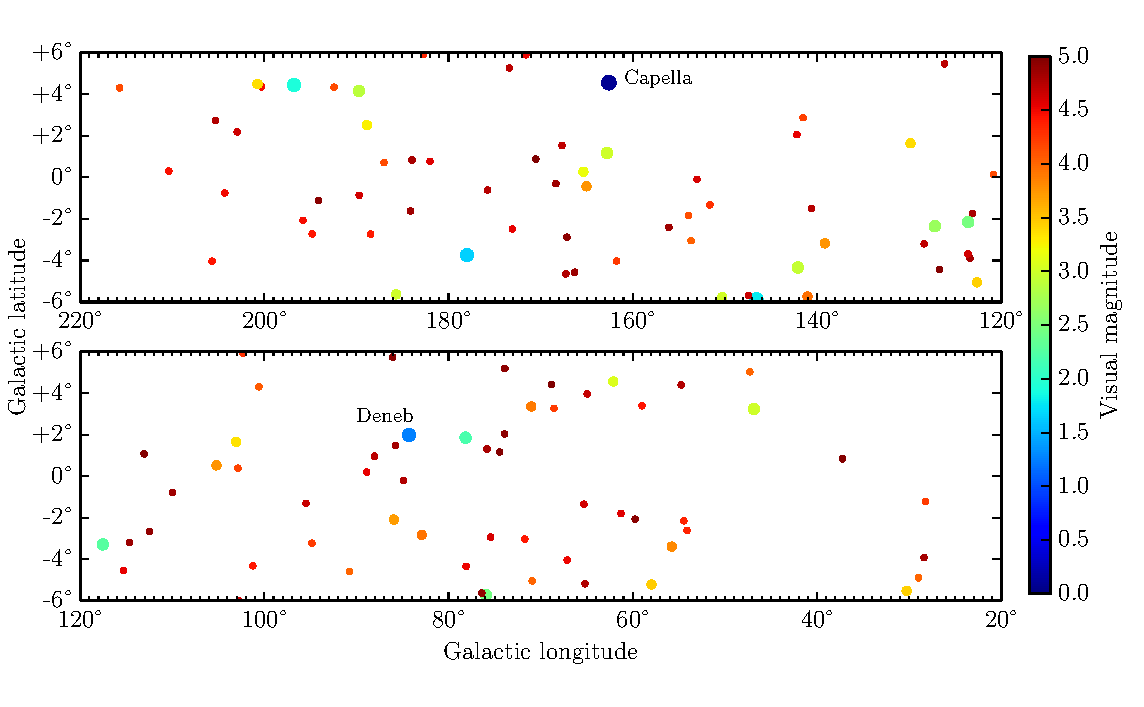
\includegraphics[width=0.9\textwidth]{figures/bright_stars.pdf} 
\caption{\footnotesize Distribution of bright ($V\leq5$) stars in the Galactic Plane, based on the catalouge of \citet{Hoffleit1991}. Symbol size, as well as colour, is scaled to visual magnitude.}
\label{fig:bright_stars}
\end{center}
\end{figure*}

\subsection{Uncertainty}
Cells which are covered by IPHAS but contain no sources (i.e. are genuinely empty down to the adopted faint limit) have an uncertainty placed on them equal to the contribution of a single source at the faint limit of the density map.

For cells covered by multiple CCDs, the availability of repeated source counts allows the impact of per-field incompleteness corrections on the reliability of the density maps to be assessed. Comparing the scaled Poisson uncertainty on the adopted cell count to the variance between counts from independently corrected CCD contributions revealed that the variance was smaller than the Poisson uncertainty in the vast majority of cases. This implies that the incompleteness correction did not introduce a significant source of uncertainty into the map; in fact the Poisson uncertainty provides a somewhat pessimistic view on the performance of the density map.

The median source count across all $r^{\prime}$-band density map cells (the distribution shown in Fig. ??) is $\approx6.2$, corresponding to $\approx20,000$ sources per sq. deg.. Assuming that over $1^{\prime}\times1^{\prime}$ cells that the source densities are uniformly distributed, on average 16\% of the area of any one cell would need to be covered in order to detect a single source - if less than this area were covered, the source count would be unreliable. Taking the expected uncertainty for an empty cell (typically $\approx1.2$ at $r^{\prime}=19$) and rounding up the minimum acceptable cell coverage fraction to 20\%, a limiting scaled error of 6 counts for an empty cell is obtained. Any unoccupied cells with greater error were discarded as being unreliable.

\subsection{Final map availability}
\begin{figure}
\begin{center}
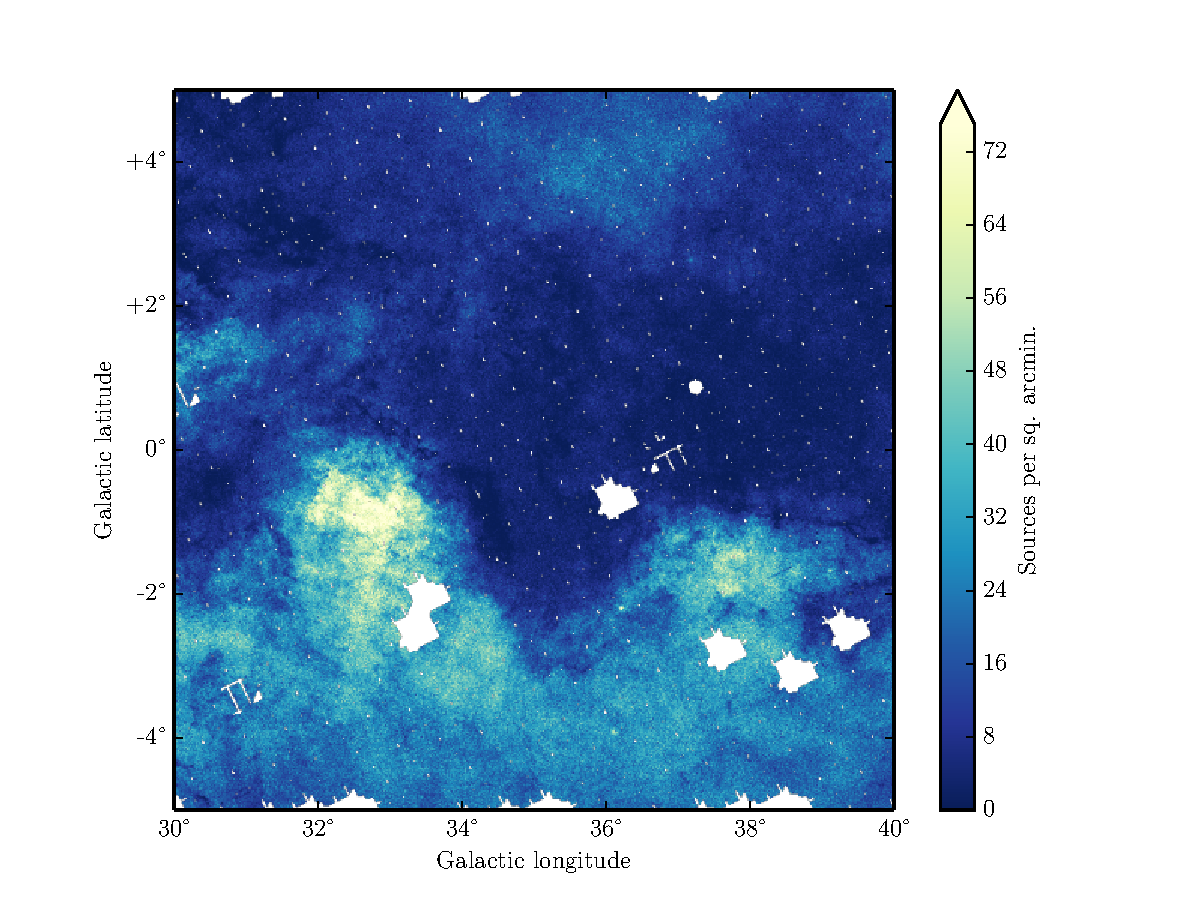
\includegraphics[width=1.0\linewidth]{figures/dmap-cutout-30-40--5-5.pdf} 
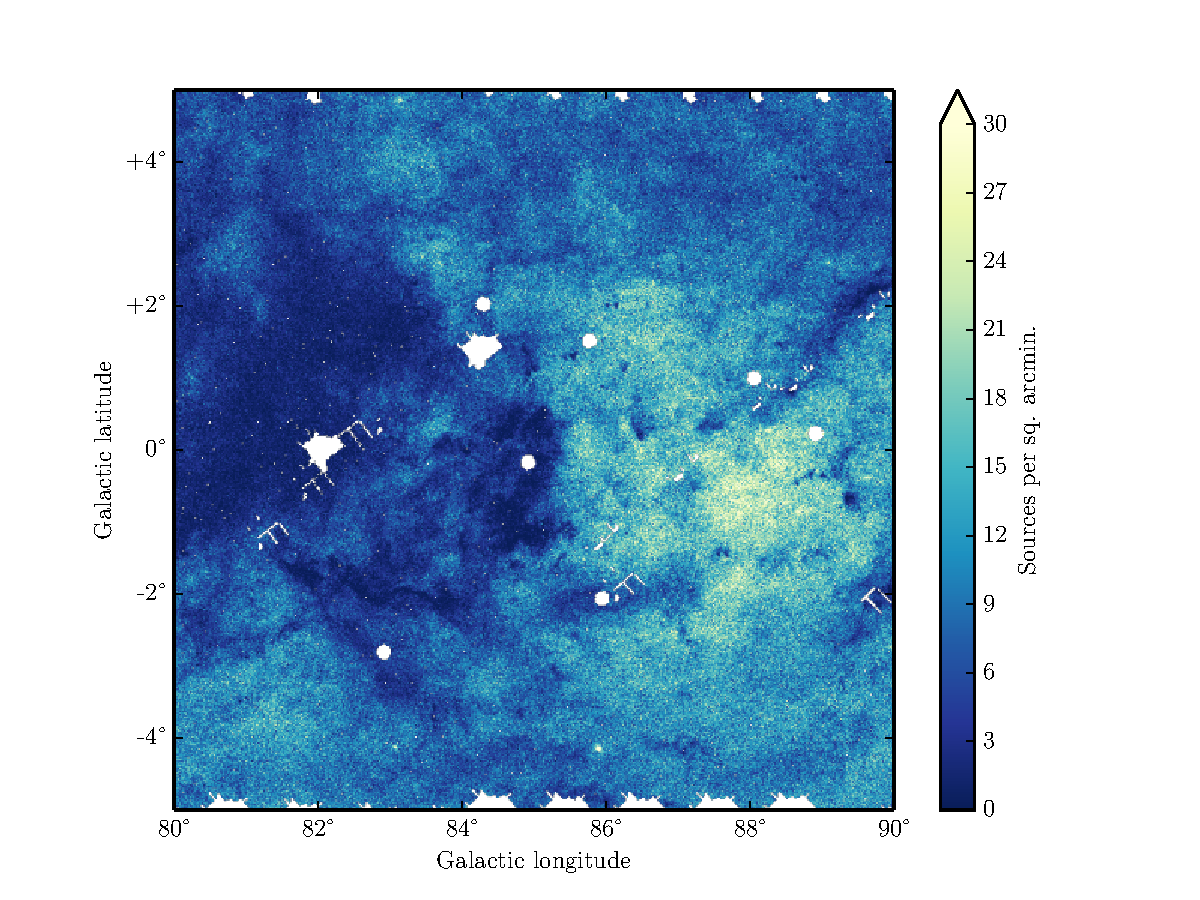
\includegraphics[width=1.0\linewidth]{figures/dmap-cutout-80-90--5-5.pdf} 
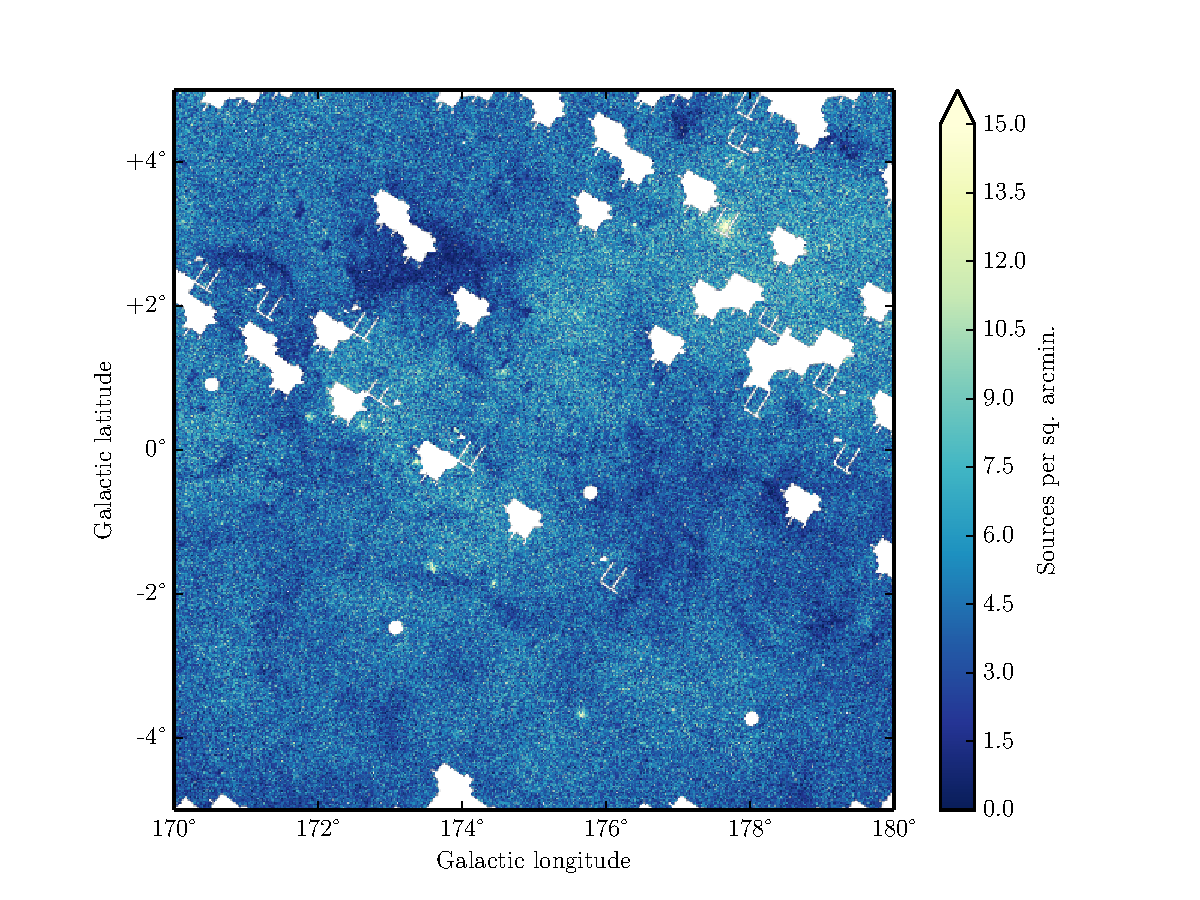
\includegraphics[width=1.0\linewidth]{figures/dmap-cutout-170-180--5-5.pdf} 
\caption{\footnotesize Cutouts of the $i^{\prime}$-band density map with $1^{\prime}\times1^{\prime}$ resolution. Upper: Inner Galaxy sightline showing the Aquila Rift. Middle: Sightline covering the Cygnus region. Lower: Anticentre sightline.}
\label{fig:dmap_cutout}
\end{center}
\end{figure}

Cutouts of the final $i^{\prime}$-band density map can be seen in Fig. \ref{fig:dmap_cutout}. The three sightlines shown illustrate the variation in stellar densities across the Galactic Plane; the inner Galaxy sightline contains some of the lowest and highest density cells in the entire map, while the $80^{\circ}<\ell<90^{\circ}$ and anticentre sightlines illustrate the declining densities towards the outer disc.

Both $r^{\prime}$- and $i^{\prime}$-band density maps are available at a variety of depths and resolutions. At each resolution the maps are stored as multi-extension FITS files, with extensions containing maps of increasingly faint limiting magnitude. Table \ref{table:fits_extensions} lists which extension corresponds to which faint limit for each band.

\begin{table}
\centering
\begin{tabular}{|c|ccccccc|}
\hline
 & 17.0 & 17.5 & 18.0 & 18.5 & 19.0 & 19.5 & 20.0  \\
\hline
$r^{\prime}$ &	- &	- &	1 &	2 &	3 &	4 &	5 \\
$i^{\prime}$ &	1 &	2 &	3 &	4 &	5 &	- &	-  \\
\hline
\end{tabular}
\caption{\footnotesize The FITS extension corresponding to faint limiting magnitudes for both $r^{\prime}$- and $i^{\prime}$-band density maps.}
\label{table:fits_extensions}
\end{table}

\section[]{Testing against models}
The Besan\c{c}on model \citep{Robin2003} is designed to generate synthetic Galactic populations, combining knowledge of the Milky Way from several sources. The model predictions are based on assumptions of a number of quantities, including density laws, star formation rates and initial mass function.

The Besan\c{c}on model is one of the tools that will be used to interpret Gaia data, and is being updated to incorporate the latest developments in studies of Galactic evolution, structure and kinematics \citep{Czekaj2014}. However the 2003 model has been used extensively \textit{(a few references)} and offers downloadable synthetic catalogues - for this reason it was adopted for comparisons against IPHAS stellar densities.


\subsection{Querying the Besan\c{c}on model}
The Besan\c{c}on model as presented in \citet{Robin2003} is made available for
use through a set of web pages\footnote{\url{http://model.obs-besancon.fr/}},
which can be used to generate synthetic catalogues based on a series of
criteria. The region over which objects are simulated can be specified in both
heliocentric distance and Galactic coordinates, extinction parameters can be
modified, spectral types and absolute magnitude ranges can be selected, and
limits based on apparent magnitudes imposed. Two output photometric systems
are available: Johnson-Cousins and CFHTLS-Megacam. Fortunately the Megacam
filters were designed to closely replicate the SDSS filter set, meaning
catalogues output by the Besan\c{c}on website can be sensibly compared with
IPHAS. The IPHAS/SDSS transformations presented in \citet{Barentsen2014} were
applied to bring the returned synthetic magnitudes into the IPHAS photometric
system.

The web interface places limits on the region of sky that can be simulated in
a single simulation, preventing the filesizes of resulting catalogues from
becoming too large. In order to simulate a significant ($>$ a few sq. deg.)
region of the Galactic Plane, a script was used to make repeated small ($\ll$1
sq. deg.) requests, moving across the area of interest, thereby building up a
larger catalogue. The diffuse extinction parameter was set to zero, allowing
custom distributions to be applied later (see Section
\ref{subsec:adding_extinction}). Querying small regions of the Galactic Plane
produced results so quickly (in a minute, roughly) that all populations of
sources were included, and the default absolute magnitude range ($-7 < M <
20$) retained. An apparent magnitude range of $8<r^{\prime}<25$ was imposed to
exclude any objects falling far outside IPHAS detection limits. Options for
including kinematics are also available but were not used here.

While the Besan\c{c}on model adopts a thin disc with a hole at its centre, its effect can be neglected as even at the lowest Galactic longitudes covered by IPHAS, the sightlines towards the inner Galaxy have their closest approach \textit{(4 kpc - check!)} to the Galactic Centre outside the affected region (their adopted hole scalelength is 1.3 kpc.).\textbf{•}

\subsection{Sightlines}

Regions of 20 sq. deg. were chosen for the comparison based on the coverage of
the density maps; areas at $\ell \approx
30^{\circ}$, $90^{\circ}$, and $175^{\circ}$ were simulated via the
Besan\c{c}on web interface, and the stellar densities of the corresponding
regions in the IPHAS $i^{\prime}$-band density maps were extracted.

\begin{figure}
\begin{center}
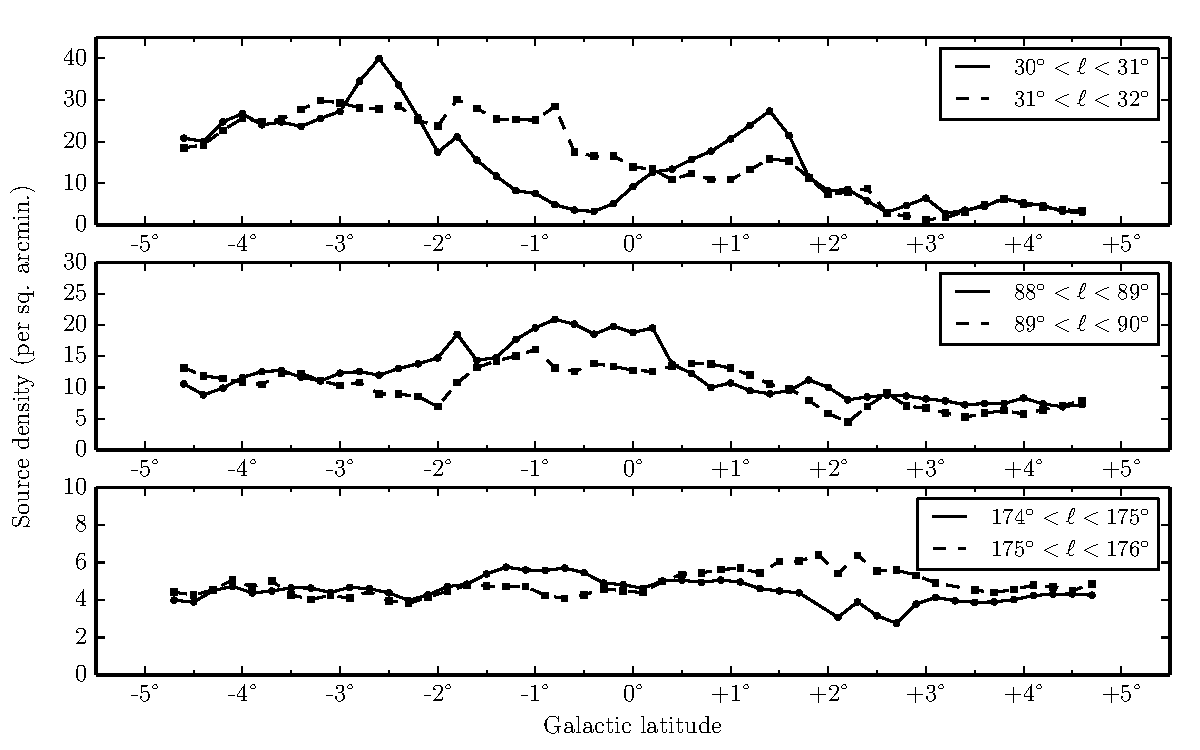
\includegraphics[width=1.0\linewidth]{figures/iphas_comparison.pdf} 
\caption{\footnotesize Stellar density profiles in Galactic latitude, averaged over $1^{\circ}$ wide strips in Galactic longitude, as given by the $20^{\prime}\times20^{\prime}$ resolution IPHAS $i^{\prime}$-band density map. Each panel shows two profiles for each sightline to be compared against star counts predicted by the Besan\c{c}on model.}
\label{fig:iphas_densities}
\end{center}
\end{figure}

Fig. \ref{fig:iphas_densities} shows the variation in stellar densities with Galactic latitude in these regions, as retrieved from the $20^{\prime}\times20^{\prime}$ resolution IPHAS $i^{\prime}$-band density map. Each sightline was split into two $1^{\circ}$-wide strips in Galactic longitude to prevent the blurring of structure in the disc; variation on these scales can be seen by comparing the densities in the two strips. Fig. \ref{fig:spiral_arms} shows the sightlines and how they relate to spiral arms according to the model of \citet{Vallee2008}.

The inner Galaxy sightline shows the largest variation with latitude and the largest variation between the two separated $1^{\circ}$-wide strips. The Aquila region ($\ell\lesssim 45^{\circ}$) contains both the highest and lowest valued cells of the entire IPHAS density map. A dark cloud at ($\approx 30^{\circ}$, $-1^{\circ}$) is responsible for the reduction in stellar density (of the amplitude $\approx 10-20$ sources per sq. arcmin.) in the $30^{\circ}<\ell <31^{\circ}$  profile relative to the $31^{\circ}<\ell <32^{\circ}$  profile. The Aquila Rift is responsible for the drop-off in stellar density at higher latitudes in both strips. Taking the spiral arm positions of \citet{Vallee2008}, it can be seen (in Fig. \ref{fig:spiral_arms}) that this sightline will pass through the Sagittarius-Carina arm twice by a distance of 10 kpc, and passes though the tangent of the Scutum-Crux arm; such spiral arm crossings are likely to render the extinction distribution in this direction quite complex.

\begin{figure}
\begin{center}
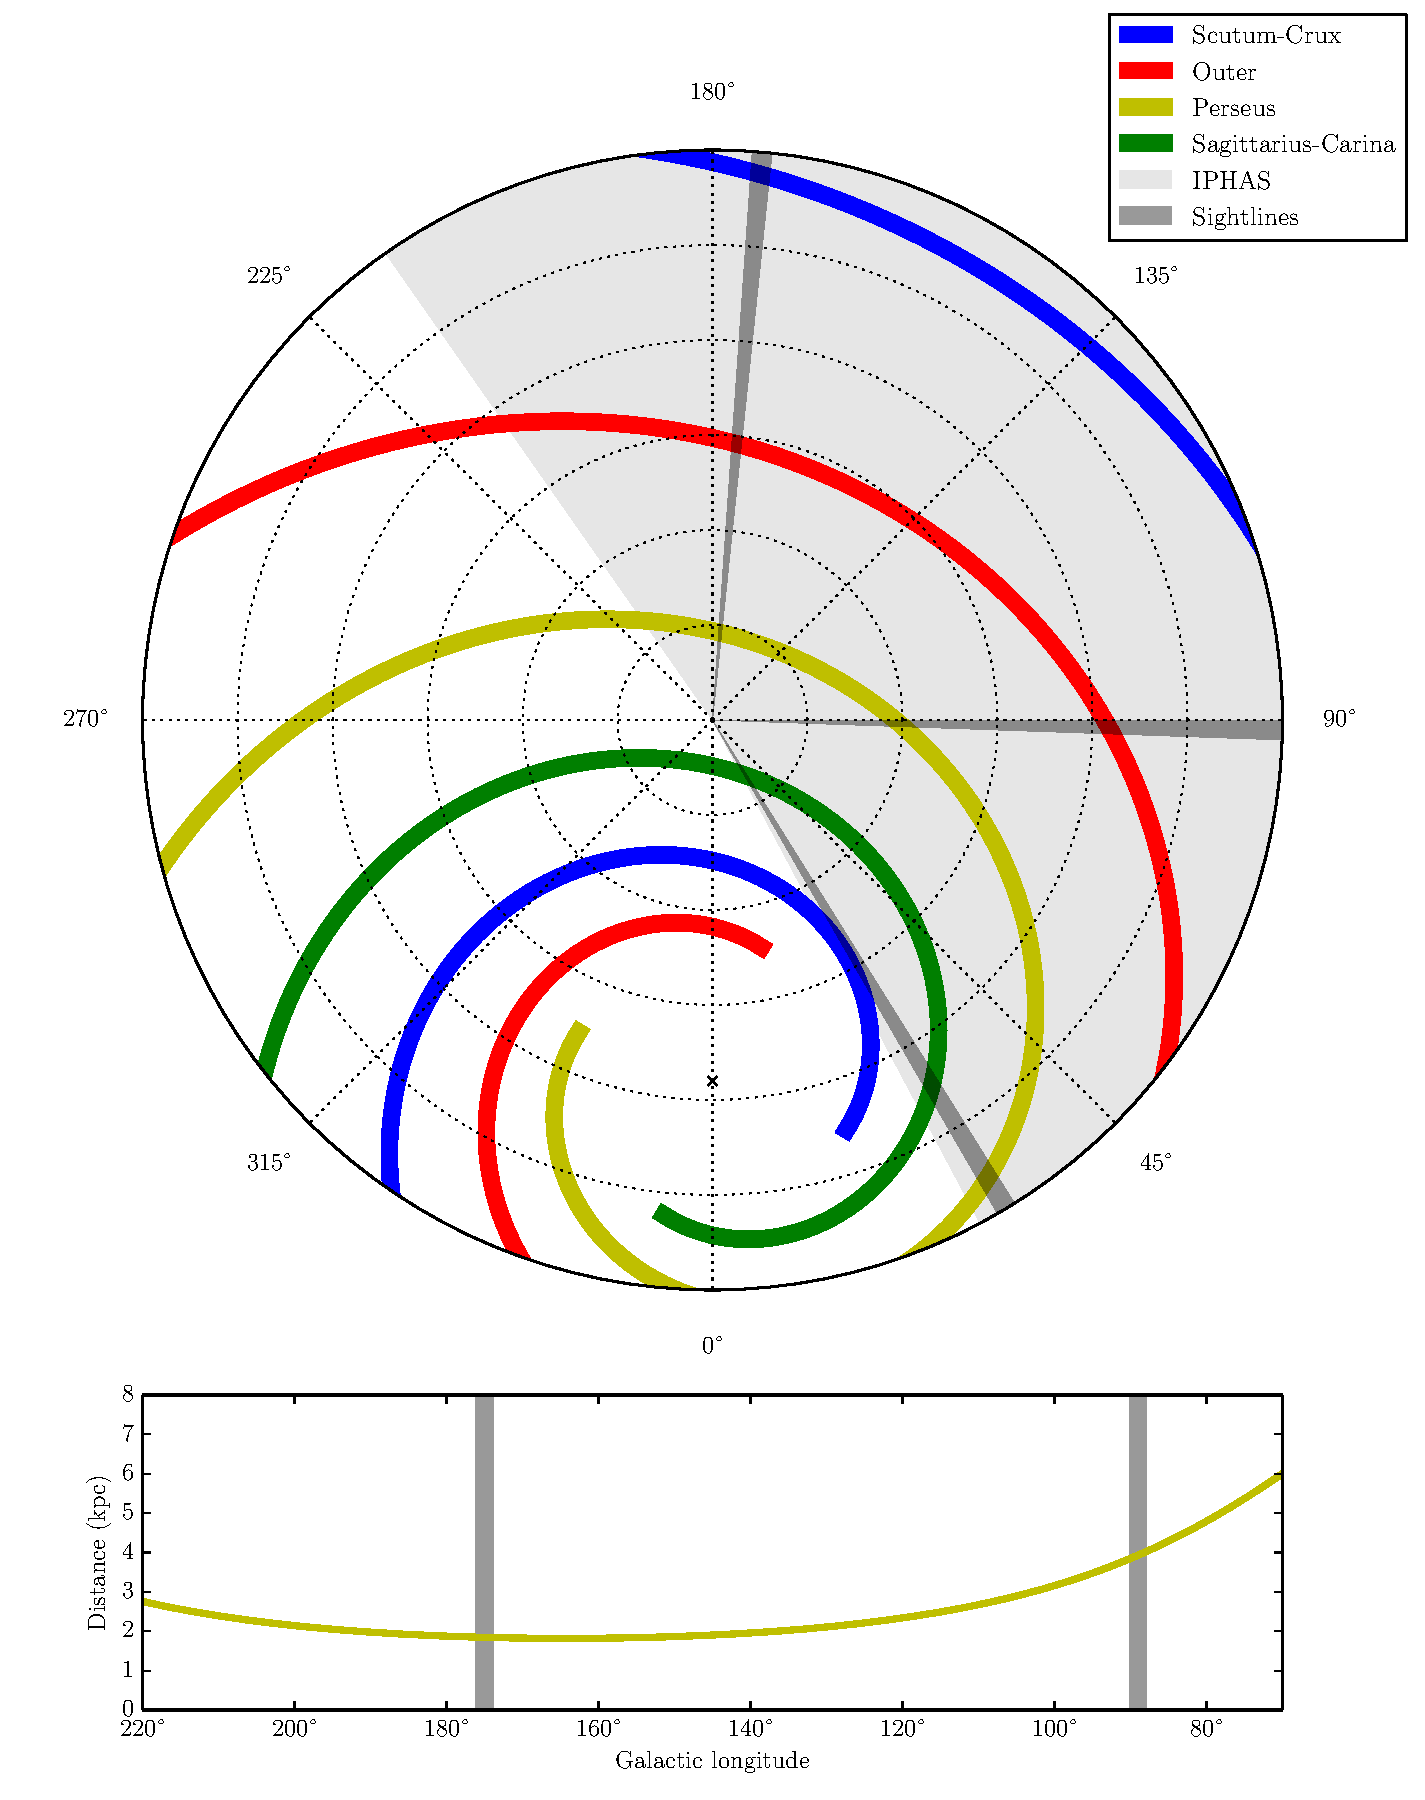
\includegraphics[width=1.0\linewidth]{figures/spiral_arms.pdf}
\caption{\footnotesize \textbf{Upper:} Distribution of spiral arms in Galactic coordinates, with distance from the Sun to the spiral arms based on the parameters obtained by \citet{Vallee2008}. Dotted circles denote distances in increments of 2 kpc. The Galactic Centre is shown as a black cross. The region covered by IPHAS is highlighted in gray. The sightlines compared with Besan\c{c}on model predictions are denoted by darker hatched regions. \textbf{Lower:} Distance to the Perseus arm in the range $70^{\circ}<\ell<220^{\circ}$ based on the parameters of \citet{Vallee2008}; this spiral arm is expected to be the main discrete feature likely to influence the observed star counts at $\ell\gtrsim 60^{\circ}$. The two IPHAS sightlines compared to Besan\c{c}on model predictions in this region are marked by gray hatched regions.}
\label{fig:spiral_arms}
\end{center}
\end{figure}

The sightline towards $\ell=90^{\circ}$, bordering the Cygnus region ($60^{\circ}\lesssim\ell\lesssim 90^{\circ}$), shows more pronounced variation with latitude, and greater variation between the two strips. Further from the Galactic midplane the two seem to be in good agreement. The spiral arm predictions of \citet{Vallee2008} place the Perseus arm at $\approx4$ kpc in this direction.

The anticentre sightline shows the least variation- at positive latitudes showing a difference of $\approx 2$ per sq. arcmin. between the two strips. The flatness of the distributions highlight the relative lack of structure apparent in the density map at these longitudes; this suggests that the Besan\c{c}on model is likely to perform well along this sightline - an exponentially decreasing stellar density with galactocentric radius has the potential to capture the observed smooth behaviour. A potential deviation from a smooth distribution comes from the Perseus Arm, predicted by \citet{Vallee2008} to lie at a distance of $\approx2$ kpc at this longitude.

\subsection{Adding extinction}
\label{subsec:adding_extinction}
With the diffuse extinction parameter set to 0 mag kpc$^{-1}$, the synthetic catalogues returned provided an unreddened view of the Milky Way. As the catalogues provide the distance to each generated object, a custom extinction profile could be imposed on the catalogued sources. Four different extinction prescriptions were applied to the catalogues, as detailed below.

\subsubsection{Marshall extinction map}
The extinction map produced by \citet{Marshall2006} were applied to the catalogues, taking the sightline closest to the synthetic catalogue coordinates - the \citet{Marshall2006} sightlines are binned in 0.25$^{\circ}$ increments in Galactic longitude and latitude. They provide curves only for sightlines with $\ell<100^{\circ}$; comparisons in the outer disc do not involve this model. The extinction in this model is given for the $K_s$ band ($A_{K_{s}}$) as a function of distance, values which were converted to $A_{i^{\prime}}$ using the extinction law of \citet{Cardelli1989} (using the conversion factors for K and I filters, giving $A_{i^{\prime}}=4.2A_{K_{s}}$).

\subsubsection{Sale extinction map}
The 3D map of \citet{Sale2014} are the result of combining IPHAS DR2 photometry with the hierarchical Bayesian model developed in \citet{Sale2012a}, which estimates the distance-extinction relationship along a given sightline, along with estimates of stellar parameters of the stars sampled. The priors adopted by this approach assume all sightlines consist entirely of thin disc stars, with a scalelength of 3 kpc.

The map provides a typical angular resolution of 10$^{\prime}$; the nearest sightline to the Besan\c{c}on catalogue under consideration was used to extinguish the synthetic photometry. While each sightline is provided with a maximum reliable distance, assuming the final value beyond these limits would result in underestimations of extinction at larger distances. For this reason, entire sightlines were used. Being based on IPHAS photometry, all the sightlines considered fall into the area covered by the map. 

\subsubsection{Perseus model}
The extinction values provided by \citet{Schlegel1998} are integrated values along the line of sight - no radial information is provided that would allow the extinguishing material to be placed along a given sightline. As a simple model of the ISM for sightlines passing through the Perseus arm, the majority of the extinction was attributed to its position, after assigning an amount of local extinction ($d < 600$ pc) based on the measurements of \citet{Lallement2014}. The location of the Perseus arm was determined from the parameters of the spiral arms obtained by \citet{Vallee2008}, as shown in Fig. \ref{fig:spiral_arms}. Taking a spiral arm half-width of 400 pc \citep{Vallee2014} and modelling the dust distribution across the arm as a Gaussian, the total extinction of \citet{Schlegel1998} (recalibrated by \citet{Schlafly2011}), less the extinction accounted for locally, was assigned across this pseudo-Perseus arm.

As illustrated by Fig. \ref{fig:spiral_arms} sightlines in the IPHAS footprint become more complicated at $\ell\lesssim 60^{\circ}$, as they pass through multiple spiral arms. For this reason the Perseus model was limited to sightlines passing through the Perseus (and potentially Outer) Arm only.

\subsubsection{Exponential disc model}
The default extinction model when using the Besan\c{c}on web interface is an exponential disc of obscuring material, with a local extinction normalisation of 0.7 mag kpc$^{-1}$ - it is noted that this value should be treated with caution in the Galactic Plane. In order to reproduce a similar extinction model, a disc of obscuring material was imposed on the Besan\c{c}on catalogue. The local A$_0$ (monochromatic extinction at 5495$\mathrm{\AA}$) normalisation was determined by imposing discs with normalisations ranging from 0 to 3 mag kpc$^{-1}$ in steps of 0.05 mag kpc$^{-1}$, to the Besan\c{c}on catalogue along each sightline. The magnitude distribution of bright ($12<r^{\prime}<15.5$) stars in the resulting extinguished synthetic catalogue was compared to the corresponding IPHAS DR2 distribution in the same area. The local normalisation that resulted in the best agreement between the two magnitude distributions was adopted for the sightline.

\subsection{Comparing IPHAS and Besan\c{c}on densities}
%\textit{Plots comparing the two, for $\approx$5 sightlines?}
\begin{figure*}
\begin{center}
\begin{flushleft}
\Large{$\ell$=30$^{\circ}$:}
\end{flushleft}

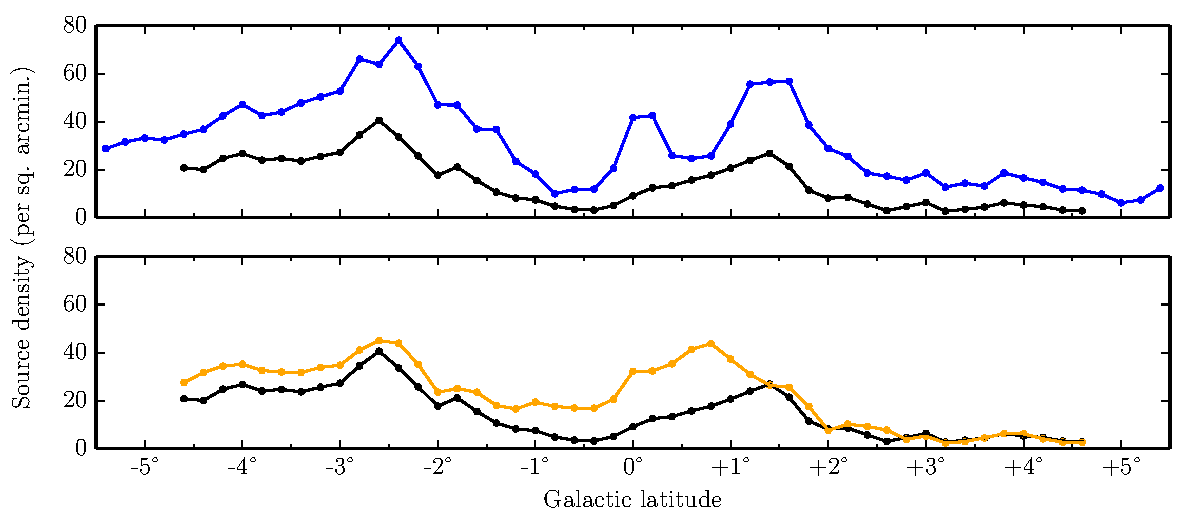
\includegraphics[width=0.9\textwidth]{figures/count_comparison_30.pdf} 

\begin{flushleft}
\Large{$\ell$=90$^{\circ}$:}
\end{flushleft}

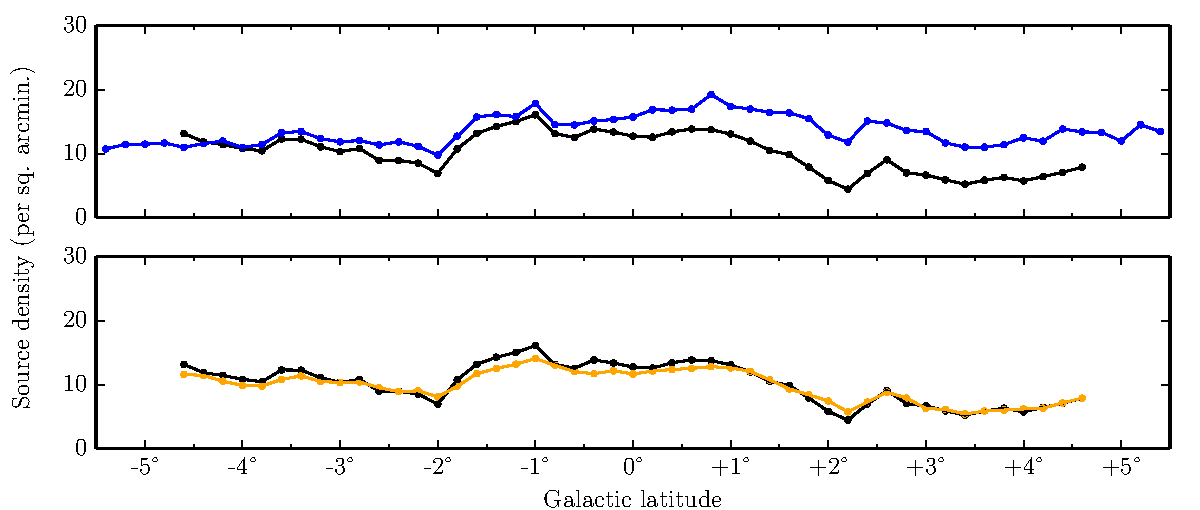
\includegraphics[width=0.9\textwidth]{figures/count_comparison_89.pdf}

\begin{flushleft}
\Large{$\ell$=175$^{\circ}$:}
\end{flushleft}

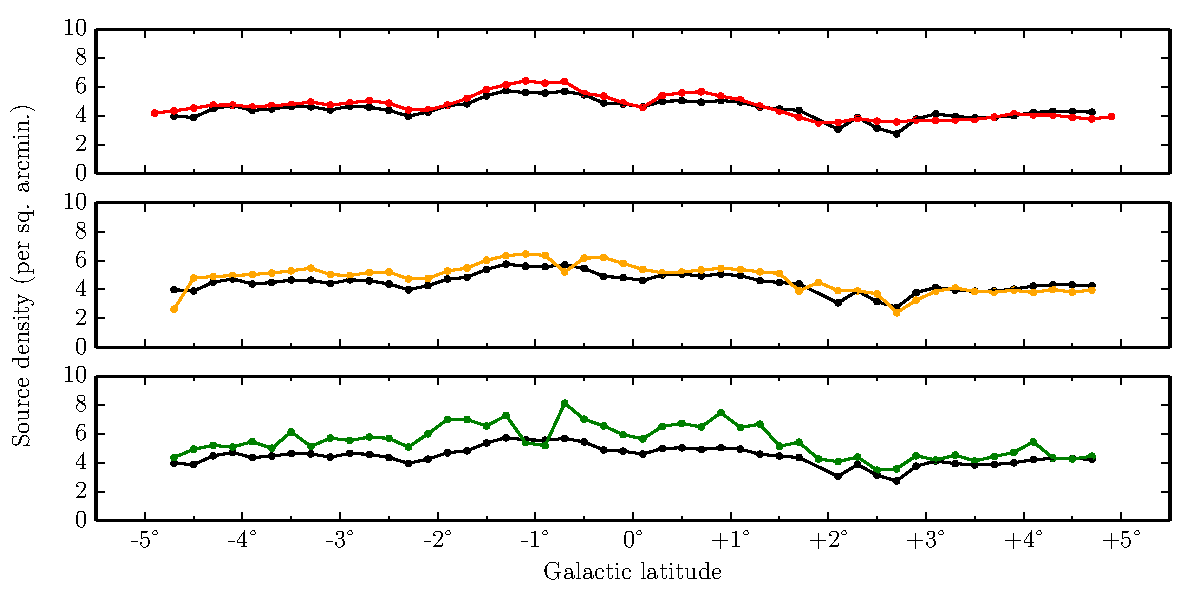
\includegraphics[width=0.9\textwidth]{figures/count_comparison_174.pdf} 
\caption{\footnotesize Comparisons between incompleteness-corrected IPHAS star counts (black) and Besan\c{c}on predictions, reddened by the extinction curves of \citet{Marshall2004} (blue) and \citet{Sale2014} (yellow). From top to bottom, comparisons are for sight lines at $\ell$=30$^{\circ}$, 90$^{\circ}$ and 175$^{\circ}$.}
\label{fig:count_comparison}
\end{center}
\end{figure*}


%\subsection{A closer look at Besan\c{c}on predictions}
%\textit{Split Besancon contributions up into spectral type, see where the majority of sources are coming from for each sightline?}

% \begin{figure*}
%  \vspace{302pt}
%  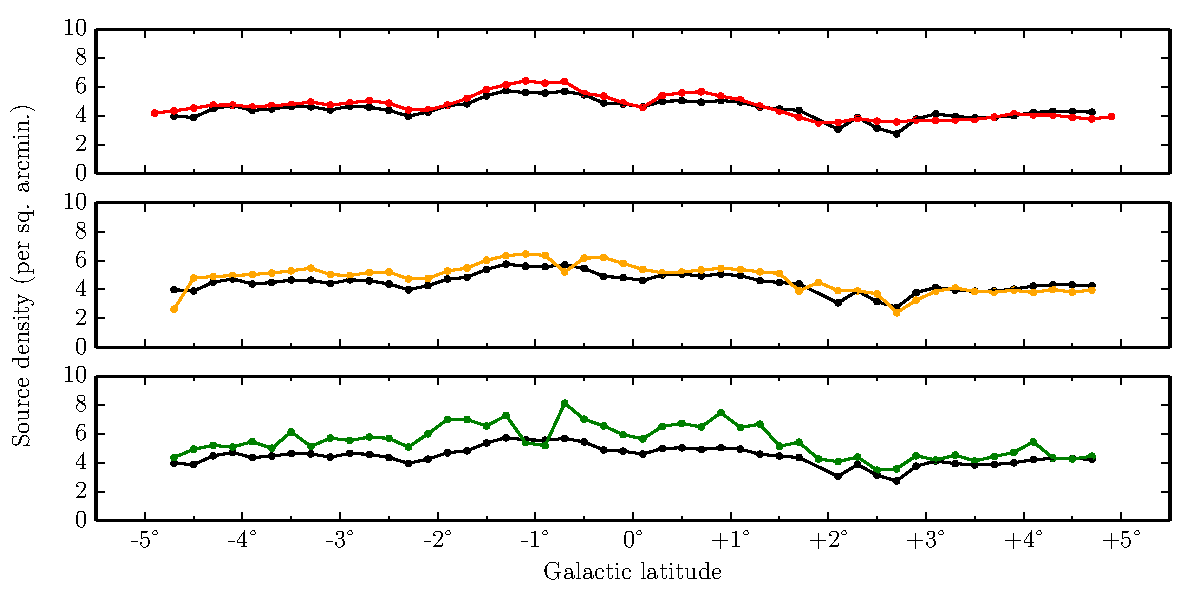
\includegraphics[width=1\textwidth]{./figures/count_comparison_174.pdf}
%  \caption{Plot of [25]--[60] colours of RV  Tauri stars against their
%   [12]--[25] colours after  normalizing as indicated in \citet{b3}.
%   Some of the objects are identified by their variable-star
%   names. Typical error bars are shown in the bottom right-hand corner.
%   The lines represent the loci for constant inner shell temperature and
%   the quantity $Q$. Note the separation of group A and B stars at $T_0
%   \sim$ 460$\,$\,K. Positions occupied by a sample of carbon and oxygen
%   Miras are also shown. The $Q=1.0$ line differs from the blackbody line
%   by a maximum of $\sim 0.05$.}
% \end{figure*}

% If we assume that the dust grains in the envelope are  predominantly of
% the same kind and are in thermal  equilibrium, the luminosity at
% frequency $\nu$ in the infrared is given by
% \begin{equation}
%    L(\nu)=\mskip-12mu\int\limits_{\rmn{envelope}}\mskip-12mu
%    \rho(r)Q_{\rmn{abs}}(\nu)B[\nu,T_{\rmn{g}}(r)]\exp [-\tau(\nu,r)]\>
%    \rmn{d}V,
% \end{equation}
%  where
%  $Q_{\rmn{abs}}(\nu)$ is the absorption efficiency at frequency $\nu$,
%  $\rho(r)$            is the dust grain density,
%  $T_{\rmn{g}}(\nu)$    is the grain temperature,
%  $B[\nu,T_{\rmn{g}}(r)]$  is the Planck function, and
%  $\tau(\nu,r)$        is the optical depth at distance {\it r\/} from the
%                       centre of the star.

% The temperature $T_{\rmn{g}}(r)$ is determined by the condition of energy
% balance: amount of energy radiated = amount of energy absorbed. The
% amount of energy absorbed at any point is proportional to the total
% available energy at that point, which consists of:
% \begin{enumerate}
%   \item the attenuated and diluted stellar radiation;
%   \item scattered radiation, and
%   \item reradiation from other grains.
% \end{enumerate}

% Detailed solutions of radiative transfer in circumstellar  dust
% shells by \citet{b21,b22} indicate that the effect of heating by
% other grains becomes significant only at large optical depths at
% the absorbing frequencies $[\tau(\rmn{UV})\gg 10]$, and at optical
% depths $\tau(\rmn{UV})<1$ the grains have approximately the same
% temperature that they would have if they were seeing the starlight
% unattenuated and no other radiation.

% The Planck mean optical depths of circumstellar envelopes  around
% several RV Tauri stars, derived from the ratios of the
% luminosities of the dust shell (at infrared wavelengths) and the
% star, range from 0.07 to 0.63 \citep{b9}. There is much
% uncertainty in the nature of the optical properties of dust grains
% in the envelope. The carbon-rich RV Tauri stars are also reported
% to show the 10-$\umu$m silicate emission feature typical of
% oxygen-rich objects \citep{b6,b19}. The pure terrestrial silicates
% or lunar silicates are found to be completely unsuitable to
% account for the infrared emission from circumstellar dust shells
% around M-type stars \citep{b21}. We assume that the absorption
% efficiency $Q_{\rmn{abs}} (\nu)$ in the infrared varies as
% $\nu^{\gamma}$. ${\gamma}=1$ appears to provide a reasonable fit
% in a variety of sources \citep*{b11,b12}. Under these
% circumstances the condition of energy balance implies that the
% dust temperature $T_{\rmn{g}}$ will vary as $r^{\beta}$.

% In view of the low value of the observed Planck mean  optical depth for
% the stellar radiation and the nature of the assumed frequency
% dependence of the absorption efficiency, the extinction of the infrared
% radiation by the dust envelope can be neglected. If we consider the
% envelope to be spherically symmetric, equation (1) reduces to
% \begin{equation}
%    L(\nu)=\!\!\int_{r_{1}}^{r_{2}}\!\!4\upi r^2\rho(r)\> Q_{\rmn{abs}}(\nu)B[\nu,T_{\rmn{g}}(r)]\> {\rmn{d}}r,
% \end{equation}
% where $r_1$ and $r_2$ are the inner and outer radii of the shell. For
% a dusty density distribution $\rho(r)\propto r^{\alpha}$ and $r_2\gg
% r_1$, equation (2) reduces to
% \begin{equation}
%    L(\nu)\propto \nu^{2+\gamma-Q}\int_{X_0}^{\infty}{{x^Q}\over
%    {\rmn{e}^x-1}}\rmn{d}x ,
% \end{equation}
% where $Q=-(\alpha+\beta+3)/\beta$ and $X_0=(h\nu /kT_0)$. $T_0$
% represents the temperature at the inner boundary of the dust shell
% where grains start condensing. In a steady radiation pressure
% driven mass outflow in the optically thin case, values of $\alpha$
% lie near $-2$ \citep{b8}. $\gamma$ and $\beta$ are related by
% $\beta=-2/(\gamma+4)$.

% In the {\it IRAS\/} Point Source Catalog \citep[PSC,][]{b2}, the
% flux densities have been quoted at the effective wavelengths 12,
% 25, 60 and \hbox{100\,$\umu$m}, assuming a flat energy spectrum
% $[\nu F(\nu)=1]$ for the observed sources. For each model given by
% equation (3), using the relative system response, the
% colour-correction factors \citep{b3} in each of the {\it IRAS\/}
% passbands were calculated and the fluxes were converted into flux
% densities expected for a flat energy distribution, as assumed in
% the {\it IRAS\/} PSC, so that the computed colours can be directly
% compared with the colours determined from the catalogue
% quantities. Such a procedure is more appropriate than correcting
% the {\it IRAS\/} colours for the energy distribution given by a
% particular model and then comparing them with those computed by
% the model.\footnote{An example of a footnote.}

% \subsection{Colour--colour diagram}

% The IR colour is defined as
% \[
%   [\nu_1]-[\nu_2]=-2.5\log [f(\nu_1)/f(\nu_2)],
% \]
%  where $\nu_1$ and $\nu_2$ are any two wavebands and $f(\nu_1)$
% and $f(\nu_2)$ are the corresponding flux  densities assuming a
% flat energy spectrum for the source. In Fig.~1, we have plotted
% the [25]--[60] colours  of RV Tauri stars against their
% corresponding [12]--[25]  colours derived from the {\it IRAS\/}
% data. Filled circles  represent stars of group A and open circles
% stars of group B. The two sets of near-parallel lines represent
% the loci of constant inner shell temperature $T_0$ and the
% quantity $Q$ defined above. The models correspond to the case of
% absorption efficiency $Q_{\rmn{abs}}(\nu)$ varying as $\nu$ (with
% $\gamma=1$ and hence $\beta=-0.4$). We have omitted R Sct in
% Fig.~1 because it shows a large deviation from the average
% relation shown by all the other objects. R Sct has a comparatively
% large excess at 60$\,\umu$m, but the extent of a possible
% contamination by the infrared cirrus \citep{b16} is unknown.
% \citet{b9} found no evidence of the presence of a dust envelope at
% near-IR wavelengths and the spectrum was consistent with a stellar
% continuum. This explains why R Sct lies well below the mean
% relation shown by stars of groups A and C between the
% [3.6]--[11.3] colour excess and the photometrically determined
% (Fe/H) \citep{b4}. R Sct has the longest period of 140$\,$d among
% the RV Tauri stars detected at far-infrared wavelengths and does
% not have the 10-$\umu$m emission feature seen in other objects
% \citep{b5,b19}. R Sct is probably the most irregular RV Tauri star
% known \citep{b17}.

% \begin{figure}
%  \vspace{302pt}
%  \caption{Plot of [25]--[60] colours of RV  Tauri stars against their
%   [12]--[25] colours after  normalizing as indicated in \citet{b3}.
%   Some of the objects are identified by their variable-star
%   names. Typical error bars are shown in the bottom right-hand corner.
%   The lines represent the loci for constant inner shell temperature and
%   the quantity $Q$. Note the separation of group A and B stars at $T_0
%   \sim$ 460$\,$\,K. Positions occupied by a sample of carbon and oxygen
%   Miras are also shown. The $Q=1.0$ line differs from the blackbody line
%   by a maximum of $\sim 0.05$.}
% \end{figure}
% The inner shell temperatures $(T_0)$ derived for the various objects
% are also given in Table~1 and we find the majority of them to have
% temperatures in the narrow range 400--600$\,$K. If the dependences of
% $Q_{\rmn{abs}}(\nu)$ on $\nu$ and $\rho(r)$ on $r$ are similar in all
% the objects considered, then in the colour--colour diagram they all
% should lie along a line corresponding to different values of $T_0$ and
% in Fig.~1 we find that this is essentially the  case. In view of the
% quoted uncertainties in the flux measurements, we cannot attach much
% significance to the scatter in Fig.~1.

% At \hbox{100\,$\umu$m} the infrared sky is characterized by
% emission, called infrared cirrus, from interstellar dust on all
% spatial scales \citep{b16}, thereby impairing the measurements at
% far-infrared wavelengths. In Fig.~2, we have plotted the
% [60]--[100] colours of the six RV Tauri stars detected at
% \hbox{100\,$\umu$m} against their [25]--[60] colours, along with
% the grid showing the regions of different values for inner shell
% temperature $T_0$ and the quantity $Q$, as in Fig.~1. The results
% indicated by Fig.~2 are consistent with those derived from Fig.~1.
% AR Pup shows a large excess at \hbox{100\,$\umu$m} but, in view of
% the large values for the cirrus flags given in the catalogue, the
% intrinsic flux at \hbox{100\,$\umu$m} is uncertain.

% \subsection{Radial distribution of dust}

% \begin{figure*}
%   \vspace*{174pt}
%   \caption{Plot of the [60]--[100] colours of RV Tauri stars against
%   their [25]--[60] colours after normalizing as indicated in \citet{b3}.
%   The solid lines represent the loci for constant
%   inner shell temperature and the quantity $Q$. The dashed line shows
%   the locus for a blackbody distribution.}
% \end{figure*}

% From Fig.~1, it is evident that all RV Tauri stars lie between the
% lines corresponding to $Q=1.5$ and 0.5. With
%  \[
%   \alpha=-(1+Q)\beta-3,
%  \]
%  these values suggest limits of $r^{-2.0}$ and $r^{-2.4}$ for the
% dust density variation, indicating a near-constant mass-loss rate.
% \citet{b12} has suggested that the density in the circumstellar
% envelope around RV Tauri stars varies as $r^{-1}$, implying a
% mass-loss rate that was greater in the past than it is currently.
% By fitting a power law to the observed fluxes, such that $f(\nu)$
% varies as $\nu^q$, values of $q$ determined by him for the various
% objects given in Table~1 lie in the range 0.6--1.2, with a mean
% $\skew5\bar q=0.98$. The assumption of a power law corresponds to
% the case of $X_0=0$ in equation (3) and hence we get
%  \[
%   q=2+\gamma -Q.
%  \]
% Since we assume that $Q_{\rmn{abs}}(\nu)$ varies as $\nu$, the
% resulting value for $Q$=2.0. None of the objects is found to lie in the
% corresponding region in the colour--colour diagram. Even this extreme
% value for $Q$ implies a density which varies as $r^{-1.8}$.

% \citet{b9} have reported that the simultaneous optical and near-IR
% data of AC Her can be fitted by a combination of two blackbodies
% at 5680 and 1800\,K, representing, respectively, the stellar and
% dust shell temperatures, and suggested that in RV Tauri stars the
% grain formation is a sporadic phenomenon and not a continuous
% process. Apparently, they have been influenced by the remark by
% \citet{b7} that their data in the 3.5--11$\,\umu$m region of AC
% Her indicated a dust temperature of $\sim$300\,K. We find that the
% {\it K--L\/} colours given by \citet{b5}, \citet{b15} and
% \citet{b9} are all consistent with each other. Surely, hot dust
% ($\sim 1800\,$K), if present at the time of observations by
% \citet{b9}, would have affected the {\it K--L\/} colour
% significantly. AC Her, like other members of its class, is found
% to execute elongated loops in the ({\it U--B\/}), ({\it B--V\/})
% plane \citep{b20}, indicating that significant departure of the
% stellar continuum from the blackbody is to be expected. Further,
% their data show only a marginal excess at the near-IR wavelengths.
% We feel that the case for the existence of hot dust around AC Her
% and hence for the sporadic grain formation around RV Tauri stars
% is not strong. In Fig.~3 we find that AC Her and RU Cen lie very
% close to R Sct which, according to \citet{b9}, shows no evidence
% for the presence of a hot dust envelope.

% \subsubsection{Comparison with oxygen and carbon Miras}

% In Fig.~1 we have also shown the positions of a sample of
% oxygen-rich and carbon-rich Miras. At the low temperatures
% characteristic of the Miras, a part of the emission at 12$\,\umu$m
% comes from the photosphere. For a blackbody at 2000$\,$K, the
% ratio of fluxes at wavelengths of 12 and 2$\,\umu$m
% $(f_{12}/f_{2})\sim 0.18$. The Miras shown in Fig.~1 have
% $(f_{12}/f_{2})$ ratios larger than twice the above value. It is
% clear that the three groups of objects populate three different
% regions of the diagram. \citet{b10} have already noticed that
% there are distinct differences between the {\it IRAS\/} colours of
% oxygen-rich and carbon-rich objects. On the basis of an analysis,
% using a bigger sample of bright giant stars in the {\it IRAS\/}
% catalogue, this has been interpreted by \citet{b25} as being due
% to a systematic difference in the dust grain emissivity index. U
% Mon shows the 10-$\umu$m silicate emission convincingly and, in
% most of the other objects for which low-resolution spectra in the
% near-infrared have been reported \citep{b5,b19}, the 10-$\umu$m
% emission may be partly attributed to silicates. Hence it is
% reasonable to expect that, in the envelopes around at least some
% of the RV Tauri stars, the dust grains are predominantly of
% silicates, as in the case of oxygen Miras \citep{b21}. The fact
% that none of the RV Tauri stars is found in the region of the
% two-colour diagram occupied by the oxygen Miras indicates that the
% emissivity indices of the silicate grains in the two cases are
% different. Because of the higher temperatures and luminosities,
% the environment of grain formation will be different in RV Tauri
% stars.

% \subsubsection{Correlation with subgroups}

% \citet{b20} have identified three spectroscopic subgroups, which
% are designated as groups A, B and C. Objects of group A are
% metal-rich; group C are metal-poor; group B objects are also
% metal-poor, but  show carbon enhancements \citep{b20,b14,b4,b1}.
% It is interesting to see that Table~1 contains no group C objects
% and that in Fig.~1 there is a clear separation of the two
% spectroscopic subgroups A and B, with the demarcation  occurring
% at an inner shell temperature of about 450$\,$K, group B stars
% having lower temperatures than group A. SX Cen is the only
% exception. \citet{b14} has reported that metal lines are stronger
% in SX Cen than in other group B objects. It may be worth noting
% that SX Cen has the shortest period among the 100 or so objects
% with the RV Tauri classification. RU Cen has the coolest inner
% shell temperature, as already suggested by the near-infrared
% spectrum \citep{b6}.
% \begin{figure}
%   \vspace*{174pt}
%   \caption{Plot of ({\it K--L\/}) colours of RV Tauri stars detected by
%   {\it IRAS\/} against their corresponding ({\it J--K\/}) colours. The
%   position of AR Pup is indicated. The three objects lying close to the
%   blackbody line are AC Her, RU Cen and R Sct.}
% \end{figure}

% Group B objects follow a different mean relationship from those of
% group A, having systematically larger 11-$\umu$m excess for a
% given excess at 3$\,\umu$m \citep{b15}. For a general sample of RV
% Tauri stars, the distinction between the oxygen-rich and
% carbon-rich objects is not that apparent in the {\it JHKL\/}
% bands. In Fig.~3 we have plotted the near-IR magnitudes of the
% objects given in Table~1 (except V Vul which has no available
% measurements) in the {\it J--K, K--L\/} plane. The colours,  taken
% from \citet{b15} and \citet{b9}, are averaged if more than one
% observation exists, because the internal agreements are found to
% be often of the order of observational uncertainties, in
% accordance with the earlier finding by \citet{b5} that variability
% has relatively little effect on colours. Barring RU Cen and AC
% Her, it is evident that stars belonging to group B show
% systematically larger excesses at {\it L\/} band for a given
% excess at {\it K}. The low excesses at near-IR wavelengths for AC
% Her and RU Cen are consistent with the very low dust temperatures
% indicated by the far-infrared colours.
% %
% \begin{figure*}
% \vbox to 220mm{\vfil Landscape figure to go here. This figure was
% not part of the original paper and is inserted here for
% illustrative purposes.\\ See the author guide for details (section
% 2.2 of \verb|mn2eguide.tex|) on how to handle landscape figures or
% tables. \caption{} \vfil} \label{landfig}
% \end{figure*}

% It is already well established that from {\it UBV\/} photometry
% one can distinguish between groups A and B,  members of group A
% being significantly redder than those of group B \citep{b20}.
% Similarly, \citet{b4} has found that the two spectroscopic groups
% are well separated in the DDO colour--colour diagrams when mean
% colours are used for the individual objects.

% The clear separation of the spectroscopic subgroups A and  B in
% the IR two-colour diagram suggests that the natures of dust grains
% in the envelopes in the two cases are not  identical. This is to
% be expected because of the differences in the physical properties
% of the stars themselves. The average colours of group B stars are
% bluer than group A, but the envelope dust temperatures of B are
% cooler than those of A. The near-IR spectra of AC Her and RU Cen
% are extremely similar \citep{b6}. The striking similarities in the
% optical spectra of AC Her and RU Cen have been pointed out by
% Bidelman \citep{b18}. We feel that the physical properties,
% including the chemical composition, of the grains  formed in the
% circumstellar envelope strongly depend on those of the embedded
% star. This, probably, explains the diversity of the energy
% distributions of RV Tauri stars in the near-infrared found by
% \citet{b6}. On the basis of the observed differences in chemical
% abundances and space distribution of RV Tauri stars, \citet{b15}
% has already pointed out that there is no direct evolutionary
% connection between group A and group B objects, thus ruling out
% the possibility that group B objects are the evolutionary
% successors of group A, in which grain formation has stopped and
% the cooler temperatures for the former are caused by an envelope
% expansion.

% \citet{b13} have subdivided RV Tauri stars into two classes, RVa
% and RVb, on the basis of their light curves; the former shows a
% constant mean  brightness, whereas the latter shows a cyclically
% varying  mean brightness. Extensive observations in the
% near-infrared show that, on average, RVb stars are redder than RVa
% stars, and \citet{b15} has suggested that in RVb stars dust shells
% are denser in the inner regions and hence radiate strongly in the
% 1--3$\,\umu$m region. Fig.~3 confirms this; RVb objects show
% systematically larger ({\it J--K\/}) and ({\it K--L\/}) colours
% than RVa objects. Apparently, there is no distinction between
% objects of the two light-curve types at far-infrared wavelengths
% (Fig.~1).

% \section{Conclusions}

% In the [12]--[25], [25]--[60] colour diagram, RV Tauri stars populate
% cooler temperature regions $(T<600 \,\rmn{K})$, distinctly different from
% those occupied by the oxygen and carbon Miras. Using a simple model
% in which
% \begin{enumerate}
%   \item the envelope is spherically symmetric,
%   \item the IR-emitting grains are predominantly of the same kind, and
%   \item in the infrared the absorption efficiency $Q_{\rmn{abs}}
%         (\nu)\propto\nu$,
% \end{enumerate}
% we find that the {\it IRAS\/} fluxes are consistent with the
% density in the envelope $\rho(r)\propto r^{-2}$, where {\it r\/}
% is the radial distance. Such a dependence for the dust density
% implies that the mass-loss rates in RV Tauri stars have not
% reduced considerably during the recent past, contrary to the
% suggestion by \citet{b12}. In the two-colour diagram, the
% blackbody line and the line corresponding to $\rho(r)\propto
% r^{-2.2}$ nearly overlap and the present data are insufficient to
% resolve between the two cases. The latter case is more physically
% reasonable, however.

% The spectroscopic subgroups A and B are well separated in  the
% {\it IRAS\/} two-colour diagram, with group B objects  having
% systematically cooler dust envelopes. If we consider only the
% objects detected by {\it IRAS}, we find that stars belonging to
% group B show systematically larger excess at {\it L\/} band for a
% given excess at {\it K}. Apparently, there is no correlation
% between the light-curve types (RVa and RVb) and the far-infrared
% behaviour of these objects. It is fairly certain that the physical
% properties, including the chemical composition, of the embedded
% stars are directly reflected by those of the dust grains. Most
% probably, the grain formation process in RV Tauri stars is
% continuous and not sporadic as suggested by \citet{b9}.

% \section*{Acknowledgments}

% I thank Professor N. Kameswara Rao for some helpful suggestions,
% Dr H. C. Bhatt for a critical reading of the original version of the
% paper and an anonymous referee for very useful comments that improved
% the presentation of the paper.


%\begin{thebibliography}{99}
\bibliographystyle{mn2e}
\bibliography{Thesis}

% \bibitem[\protect\citeauthoryear{Baird}{1981}]{b1} Baird S.R., 1981,
% ApJ, 245, 208
% \bibitem[\protect\citeauthoryear{Beichman et al.}{1985a}]{b2} Beichman
% C.A., Neugebauer G., Habing H.J., Clegg P.E., Chester T.J., 1985a,
% {\it IRAS\/} Point Source Catalog. Jet Propulsion Laboratory,
% Pasadena
% \bibitem[\protect\citeauthoryear{Beichman et al.}{1985b}]{b3} Beichman
% C.A., Neugebauer G., Habing H.J., Clegg P.E., Chester T.J., 1985b,
% {\it IRAS\/} Explanatory Supplement. Jet Propulsion Laboratory,
% Pasadena
% \bibitem[\protect\citeauthoryear{Dawson}{1979}]{b4} Dawson D.W., 1979,
% ApJS, 41, 97
% \bibitem[\protect\citeauthoryear{Gerhz}{1972}]{b5} Gerhz R.D., 1972, ApJ,
% 178, 715
% \bibitem[\protect\citeauthoryear{Gerhz \& Ney}{1972}]{b6} Gerhz R.D., Ney
% E.P., 1972, PASP, 84, 768
% \bibitem[\protect\citeauthoryear{Gerhz \& Woolf}{1970}]{b7} Gerhz R.D., Woolf N.J.,
% 1970, ApJ, 161, L213
% \bibitem[\protect\citeauthoryear{Gilman}{1972}]{b8} Gilman R.C., 1972, ApJ, 178, 423
% \bibitem[\protect\citeauthoryear{Goldsmith et al.}{1987}]{b9} Goldsmith M.J., Evans A.,
% Albinson J.S., Bode M.F., 1987, MNRAS, 227, 143
% \bibitem[\protect\citeauthoryear{Hacking et al.}{1985}]{b10} Hacking P. et al., 1985,
% PASP, 97, 616
% \bibitem[\protect\citeauthoryear{Harvey, Thronson \& Gatley}{Harvey et al.}{1979}]{b11}
% Harvey P.M., Thronson H.A., Gatley I., 1979, ApJ, 231, 115
% \bibitem[\protect\citeauthoryear{Jura}{1986}]{b12} Jura M., 1986, ApJ, 309, 732
% \bibitem[\protect\citeauthoryear{Kukarkin et al.}{1969}]{b13} Kukarkin B.V. et al.,
% 1969, General Catalogue of Variable Stars. Moscow
% \bibitem[\protect\citeauthoryear{Lloyd Evans}{1974}]{b14} Lloyd Evans T., 1974, MNRAS,
% 167, 17{\sc p}
% \bibitem[\protect\citeauthoryear{Lloyd Evans}{1985}]{b15} Lloyd Evans T., 1985, MNRAS,
% 217, 493
% \bibitem[\protect\citeauthoryear{Low et al.}{1984}]{b16} Low F.J. et al., 1984, ApJ,
% 278, L19
% \bibitem[\protect\citeauthoryear{McLaughlin}{1932}]{b17} McLaughlin D.B., 1932, Publ. Univ.
% Obs. Mich., 4, 135
% \bibitem[\protect\citeauthoryear{O'Connell}{1961}]{b18} O'Connell J.K., 1961, Specola
% Vaticana Ric. Astron., 6, 341
% \bibitem[\protect\citeauthoryear{Olnon \& Raimond}{1986}]{b19} Olnon F.M., Raimond E., 1986,
% A\&AS, 65, 607
% \bibitem[\protect\citeauthoryear{Preston et al.}{1963}]{b20} Preston G.W., Krzeminski W., Smak J.,
% Williams J.A., 1963, ApJ, 137, 401
% \bibitem[\protect\citeauthoryear{Rowan-Robinson \& Harris}{1983a}]{b21} Rowan-Robinson M., Harris
% S., 1983a, MNRAS, 202, 767
% \bibitem[\protect\citeauthoryear{Rowan-Robinson \& Harris}{1983b}]{b22} Rowan-Robinson M., Harris
% S., 1983b, MNRAS, 202, 797
% \bibitem[\protect\citeauthoryear{van der Veen \& Habing}{1988}]{b23} van der Veen W.E.C.J., Habing
% H.J., 1988, A\&A, 194, 125
% \bibitem[\protect\citeauthoryear{Willems \& de Jong}{1988}]{b24} Willems F.J., de Jong T., 1988,
% A\&A, 196, 173
% \bibitem[\protect\citeauthoryear{Zuckerman \& Dyck}{1986}]{b25} Zuckerman B., Dyck H.M., 1986, ApJ,
% 311, 345
%\end{thebibliography}

\appendix

\section[]{Artificial object insertion for testing completeness}
\textsl{Algorithm / figure showing processing steps}

\section[]{IPHAS/GAIA transformations}
\textsl{Could be useful?}


% (This appendix was not part of the original paper by
% A.V.~Raveendran and is included here just for illustrative
% purposes. The references are not relevant to the text of the
% appendix, they are references from the bibliography used to
% illustrate text before and after citations.)

% Spectroscopic observations of bright quasars show that the mean
% number density of Ly$\alpha$ forest lines, which satisfy certain
% criteria, evolves like $\rmn{d}N/\rmn{d}z=A(1+z)^\gamma$, where
% $A$ and~$\gamma$ are two constants.  Given the above intrinsic
% line distribution we examine the probability of finding large gaps
% in the Ly$\alpha$ forests.  We concentrate here only on the
% statistics and neglect all observational complications such as the
% line blending effect \citep[see][for example]{b11}.

% Suppose we have observed a Ly$\alpha$ forest between redshifts $z_1$
% and~$z_2$ and found $N-1$ lines.  For high-redshift quasars $z_2$~is
% usually the emission redshift $z_{\rmn{em}}$ and $z_1$ is set to
% $(\lambda_{\rmn{Ly}\beta}/\lambda_{\rmn{Ly}\alpha})(1+z_{\rmn{em}})=0.844
% (1+z_{\rmn{em}})$ to avoid contamination by Ly$\beta$ lines.  We
% want to know whether the largest gaps observed in the forest are
% significantly inconsistent with the above line distribution.  To do
% this we introduce a new variable~$x$:
% %
% \begin{equation}
% x={(1+z)^{\gamma+1}-(1+z_1)^{\gamma+1} \over
%      (1+z_2)^{\gamma+1}-(1+z_1)^{\gamma+1}}.
% \end{equation}
% %
% $x$ varies from 0 to 1.  We then have $\rmn{d}N/\rmn{d}x=\lambda$, where $\lambda$
% is the mean number of lines between $z_1$ and $z_2$ and is given by
% %
% \begin{equation}
% \lambda\equiv{A[(1+z_2)^{\gamma+1}-(1+z_1)^{\gamma+1}]\over\gamma+1}.
% \end{equation}
% %
% This means that the Ly$\alpha$ forest lines are uniformly
% distributed in~$x$. The probability of finding $N-1$ lines between $z_1$
% and~$z_2$, $P_{N-1}$, is assumed to be the Poisson distribution.
% %
% \newpage
% %
% \begin{figure}
% \vspace{11pc}
% \caption{$P(>x_{\rmn{gap}})$ as a function of $x_{\rmn{gap}}$ for,
%  from left to right, $N=160$, 150, 140, 110, 100, 90, 50, 45 and~40.
%  Compare this with \protect\citet{b15}.}
% \label{appenfig}
% \end{figure}

% \subsection{Subsection title}

% We plot in Fig.~\ref{appenfig} $P(>x_{\rmn{gap}})$ for several $N$
% values. We see that, for $N=100$ and $x_{\rmn{gap}}=0.06$,
% $P(>0.06)\approx20$ per cent.  This means that the probability of
% finding a gap with a size larger than six times the mean
% separation is not significantly small. When the mean number of
% lines is large, $\lambda\sim N>>1$, our $P(>x_{\rmn{gap}})$
% approaches the result obtained by \citet[fig. 4]{b22} for small
% (but still very large if measured in units of the mean separation)
% $x_{\rmn{gap}}$, i.e., $P(>x_{\rmn{gap}})\sim N(1-
% x_{\rmn{gap}})^{N-1}\sim N {\rmn{exp}}(-\lambda x_{\rmn{gap}})$.

% \bsp

\label{lastpage}

\end{document}
